\documentclass[12pt,a4paper]{article}

% ============================================================
% IDIOMA Y TIPOGRAFÍA
% ============================================================
\usepackage[utf8]{inputenc}
\usepackage[T1]{fontenc}
\usepackage[spanish,es-nodecimaldot]{babel}
\usepackage{lmodern}
\usepackage{microtype}
\usepackage{csquotes}

\addto\captionsspanish{%
  \renewcommand{\tablename}{Tabla}%
  \renewcommand{\figurename}{Figura}%
}

% ============================================================
% FORMATO DE PÁGINA
% ============================================================
\usepackage[
  top=2.54cm,
  bottom=2.54cm,
  left=2.54cm,
  right=2.54cm
]{geometry}

\usepackage{setspace}
\setstretch{1.15}

\setlength{\parindent}{1.27cm}
\setlength{\parskip}{0pt}
\setlength{\emergencystretch}{3em}

% ============================================================
% MATEMÁTICA, TABLAS Y FIGURAS
% ============================================================
\usepackage{amsmath}
\usepackage{amssymb}
\usepackage{graphicx}
\usepackage{float}
\usepackage{booktabs}
\usepackage{multirow}
\usepackage{threeparttable}
\usepackage{array}
\usepackage{tabularx}
\usepackage{xurl}

\graphicspath{{../figures/}}

\usepackage{caption}
\captionsetup{
  font=small,
  labelfont=bf,
  labelsep=newline,
  justification=raggedright,
  singlelinecheck=false,
  skip=5pt
}

\setlength{\textfloatsep}{10pt plus 2pt minus 2pt}
\setlength{\floatsep}{8pt plus 2pt minus 2pt}
\setlength{\intextsep}{8pt plus 2pt minus 2pt}

% ============================================================
% BIBLIOGRAFÍA APA 7
% ============================================================
\usepackage[
  backend=biber,
  style=apa,
  sorting=nyt,
  sortcites=true,
  maxcitenames=2,
  maxbibnames=20
]{biblatex}

\DeclareLanguageMapping{spanish}{spanish-apa}

\DefineBibliographyStrings{spanish}{
  andothers = {et\addabbrvspace al\adddot}
}

\addbibresource{referencias.bib}
\setlength{\bibitemsep}{0.5\baselineskip}

% ============================================================
% ENCABEZADO Y PIE DE PÁGINA
% ============================================================
\usepackage{fancyhdr}

\pagestyle{fancy}
\fancyhf{}

\fancyhead[L]{\footnotesize\itshape Convergencia regional en el Perú}
\fancyhead[R]{\footnotesize Karen A. Medrano Valenzuela}

\fancyfoot[C]{\small\thepage}

\setlength{\headheight}{15pt}
\setlength{\footskip}{26pt}

\renewcommand{\headrulewidth}{0.4pt}
\renewcommand{\footrulewidth}{0pt}

% ============================================================
% ENLACES
% ============================================================
\usepackage[hidelinks]{hyperref}
\urlstyle{same}

% ============================================================
% DOCUMENTO
% ============================================================
\begin{document}

\thispagestyle{plain}

\begin{center}
{\Large\bfseries
Disparidades socioeconómicas y convergencia regional en el Perú:
un análisis de heterogeneidad espacial, 2007--2019
\par}

\vspace{0.6em}

{\normalsize Karen Aymé Medrano Valenzuela\par}
{\normalsize Universidad Nacional de San Cristóbal de Huamanga\par}
{\normalsize Facultad de Ciencias Económicas, Administrativas y Contables\par}
\end{center}

\vspace{0.5em}

\section*{Resumen}

El objetivo de esta investigación es analizar la evolución de las disparidades
socioeconómicas y la convergencia regional en el Perú durante el periodo
2007--2019, considerando las posibles heterogeneidades espaciales existentes
entre los departamentos. El estudio comprende 24 departamentos y emplea dos
indicadores: el Índice de Desarrollo Humano y el producto bruto interno real
per cápita relativo. La estrategia empírica combina estadística descriptiva,
densidades kernel, análisis cartográfico, el índice global de Moran, regresiones
de convergencia beta mediante mínimos cuadrados ordinarios, modelos de error
espacial, especificaciones Durbin de error y regresiones geográficamente
ponderadas.

Los resultados evidencian comportamientos diferenciados. En el caso del
desarrollo humano, el coeficiente asociado con el nivel inicial es positivo y
estadísticamente significativo, por lo que no se identifica convergencia beta
durante el periodo analizado. Aunque la dispersión relativa del IDH disminuye,
los departamentos con mayores niveles iniciales registraron incrementos
superiores. En contraste, el coeficiente del PBI real per cápita relativo
inicial es negativo y altamente significativo, lo que revela un proceso de
convergencia económica regional. Los índices globales de Moran no muestran
autocorrelación espacial estadísticamente significativa; sin embargo, la
regresión geográficamente ponderada identifica diferencias territoriales en la
intensidad de la convergencia económica. En conjunto, los resultados sugieren
que la reducción de las brechas de ingreso no necesariamente estuvo acompañada
por una convergencia equivalente en las dimensiones del desarrollo humano.

\vspace{0.3cm}

\noindent\textbf{Palabras clave:} convergencia regional; desarrollo humano;
PBI per cápita; econometría espacial; heterogeneidad espacial; Perú.

\vspace{0.4cm}

\noindent\textbf{Clasificación JEL:} C21, O18, O47, R11, R12.

\section{Introducción}

Las desigualdades territoriales representan una de las expresiones más evidentes
del desarrollo económico desigual. Aun cuando las regiones de un mismo país
comparten un mismo marco institucional y macroeconómico, pueden seguir
trayectorias muy distintas en términos de ingreso, productividad, educación,
salud y condiciones de vida. Esto significa que el crecimiento del producto por
habitante no siempre se traduce en mejoras similares para toda la población.
En este sentido, el análisis del desarrollo regional requiere considerar tanto los
aspectos económicos como los factores sociales que influyen en las oportunidades
y capacidades de las personas.

La teoría neoclásica del crecimiento plantea que las economías con menores
niveles iniciales de capital e ingreso pueden crecer a un ritmo más acelerado,
debido a los rendimientos marginales decrecientes del capital
\parencite{solow1956}. Bajo este enfoque, la convergencia beta ocurre cuando las
regiones inicialmente rezagadas presentan tasas de crecimiento superiores a las
de aquellas con mayores niveles de desarrollo. Esta idea fue contrastada de
manera empírica por \textcite{barro_sala1991} y
\textcite{barro_sala1992}, y posteriormente ampliada con la incorporación del
capital humano y otros factores estructurales
\parencite{mankiw1992}.

Un coeficiente negativo entre el nivel inicial y el crecimiento posterior no
demuestra, por sí mismo, que las brechas regionales estén disminuyendo.
\textcite{quah1993} advierte que las regresiones tradicionales de convergencia
pueden ocultar transformaciones en la distribución, persistencia de
desigualdades e incluso la formación de grupos de regiones con trayectorias
diferenciadas. De ahí la necesidad de complementar la estimación beta con
medidas de dispersión, densidades kernel y otros procedimientos que permitan
examinar la evolución de la distribución en su conjunto.

La dimensión espacial añade un elemento central al análisis. Las regiones no
siguen trayectorias independientes, pues mantienen relaciones económicas,
productivas, laborales y geográficas con los territorios próximos. La
localización de la infraestructura, la concentración de actividades
económicas, el acceso a los mercados y las economías de aglomeración pueden
reforzar las ventajas de determinados espacios \parencite{krugman1991}.
Prescindir de estas interacciones podría generar estimaciones incompletas y
lecturas poco representativas de la organización territorial de la economía
\parencite{anselin1988,rey_montouri1999}.

La interpretación de las desigualdades regionales también cambia según el
indicador seleccionado. El ingreso per cápita aproxima la capacidad económica
promedio de un territorio, aunque no resume adecuadamente sus condiciones de
salud, educación y bienestar. Desde el enfoque de las capacidades, el
desarrollo se relaciona con la ampliación de las libertades reales de las
personas y no únicamente con el incremento de sus ingresos
\parencite{sen1999}. Bajo esta perspectiva, la investigación examina
conjuntamente el PBI real per cápita relativo y el Índice de Desarrollo Humano.
La comparación permite establecer si el acercamiento económico entre
departamentos estuvo acompañado por una reducción semejante de las brechas
sociales.

La evidencia internacional indica, además, que la convergencia puede presentar
intensidades distintas dentro de un mismo país. El estudio de
\textcite{duran2024} sobre las regiones de Turquía combina indicadores
socioeconómicos, econometría espacial y regresiones geográficamente ponderadas,
y encuentra que los parámetros estimados varían territorialmente. El presente
trabajo retoma esa estrategia para el caso peruano, con adecuaciones derivadas
de la disponibilidad de información, el periodo de estudio y la escala
departamental de las variables.

En el Perú, las diferencias acumuladas en infraestructura, capital humano,
estructura productiva, urbanización y acceso a los mercados justifican una
lectura explícitamente territorial. Algunos departamentos concentran
actividades de mayor productividad y una oferta más amplia de servicios,
mientras otros todavía enfrentan restricciones estructurales que limitan la
generación de ingresos y la ampliación de capacidades. Una evaluación basada
solo en promedios nacionales podría ocultar tanto la magnitud de estas brechas
como la diversidad de las trayectorias departamentales.

Sobre esta base, la investigación plantea la siguiente pregunta: ¿existió
convergencia regional en desarrollo humano y PBI real per cápita relativo
entre los departamentos del Perú durante 2007--2019, y en qué medida dicho
proceso presentó heterogeneidad espacial? El objetivo general es analizar las
disparidades socioeconómicas y la convergencia regional a partir de la
distribución de los indicadores, la autocorrelación espacial y la variación
territorial de los coeficientes estimados.

La estrategia empírica combina estadísticos descriptivos, densidades kernel,
mapas temáticos, el índice global de Moran, regresiones de convergencia beta
mediante mínimos cuadrados ordinarios, modelos de error espacial,
especificaciones Durbin de error y regresiones geográficamente ponderadas. Los
hallazgos revelan trayectorias diferentes entre las dos dimensiones
consideradas. El PBI real per cápita relativo presenta evidencia de
convergencia beta, mientras que el IDH mantiene una relación positiva entre su
nivel inicial y el cambio posterior. La heterogeneidad territorial también es
más marcada en la convergencia económica que en la evolución del desarrollo
humano.

El artículo se divide en seis secciones. Luego de esta introducción, la segunda
sección desarrolla la revisión de literatura y los fundamentos teóricos. La
tercera presenta las fuentes de información y el procedimiento metodológico.
La cuarta reúne los resultados descriptivos, espaciales y econométricos. La
quinta discute los principales hallazgos, sus implicancias y las limitaciones
del estudio. La última sección expone las conclusiones.

\section{Revisión de literatura}

\subsection{Convergencia económica regional}

La hipótesis de convergencia regional sostiene que las economías que parten de
niveles más bajos de desarrollo pueden crecer con mayor rapidez que aquellas
que se encuentran inicialmente mejor posicionadas. En el modelo neoclásico,
esta posibilidad se explica por los rendimientos marginales decrecientes del
capital: manteniendo constantes las demás condiciones, una unidad adicional de
inversión genera un retorno relativamente mayor en los territorios con menor
dotación inicial \parencite{solow1956}. Esta proposición fue trasladada al
análisis empírico por \textcite{barro_sala1991} y
\textcite{barro_sala1992}, quienes examinaron la relación entre el nivel
inicial de ingreso y el crecimiento posterior de las economías.

A partir de este enfoque se distinguen dos formas de convergencia. La
convergencia beta se presenta cuando existe una relación negativa entre el
nivel inicial del indicador y su variación posterior; en otras palabras, las
regiones rezagadas crecen, en promedio, a una tasa superior a la de las
regiones inicialmente más desarrolladas. La convergencia sigma, en cambio, se
refiere a la disminución de la dispersión entre territorios a lo largo del
tiempo. Aunque ambas nociones están vinculadas, responden a preguntas
diferentes. La primera analiza la influencia de las condiciones iniciales sobre
el crecimiento, mientras que la segunda observa si la distribución regional se
vuelve efectivamente menos desigual. Por ello, la presencia de convergencia
beta no asegura, por sí sola, una reducción de las brechas.

La ampliación del modelo neoclásico incorporó posteriormente el papel del
capital humano. \textcite{mankiw1992} muestran que la educación, las
capacidades productivas y la acumulación de conocimientos ayudan a explicar por
qué regiones con niveles iniciales de ingreso semejantes pueden seguir
trayectorias distintas. Las diferencias en salud, infraestructura, formación
laboral o calidad institucional condicionan la capacidad de cada territorio
para sostener el crecimiento. En ese contexto, la convergencia absoluta pierde
fuerza como supuesto general, sobre todo cuando las regiones presentan
estructuras económicas y sociales marcadamente heterogéneas.

\subsection{Distribución, polarización y clubes de convergencia}

El enfoque tradicional de la convergencia beta ha recibido diversas críticas,
ya que resume el comportamiento de todas las regiones mediante un único
coeficiente promedio. Según \textcite{quah1993}, una relación negativa entre el
nivel inicial de ingreso y el crecimiento posterior no implica necesariamente
que las diferencias regionales estén desapareciendo. Es posible que persistan
brechas importantes, que exista una limitada movilidad entre regiones o incluso
que se produzca un proceso de polarización. En estos casos, las economías no
convergen hacia un mismo estado de equilibrio, sino que pueden agruparse en
diferentes estados estacionarios.

A partir de este planteamiento surge el concepto de clubes de convergencia. Bajo
este enfoque, algunas regiones logran converger entre sí, mientras mantienen
diferencias persistentes respecto a otros grupos. La presencia de distribuciones
multimodales o de los denominados ``picos gemelos'' suele interpretarse como un
indicio de polarización regional \parencite{quah1996}. Por esta razón, las
regresiones de convergencia suelen complementarse con medidas de dispersión,
estimaciones de densidad kernel y métodos no paramétricos, los cuales permiten
analizar cómo evoluciona la distribución completa de los indicadores y no solo
su promedio.

Esta diferencia adquiere especial importancia cuando el análisis se realiza con
indicadores de desarrollo humano. Una reducción de las brechas de ingreso no
significa necesariamente que también mejoren de manera similar la salud, la
educación o las condiciones de vida de la población. Desde el enfoque de las
capacidades, el desarrollo debe entenderse como la ampliación de las libertades
y oportunidades reales de las personas, más allá del crecimiento del ingreso o
del valor monetario de la producción \parencite{sen1999}. En ese sentido,
comparar el PBI per cápita con el IDH permite evaluar si el acercamiento
económico entre las regiones estuvo acompañado por una convergencia en términos
de desarrollo humano.

\subsection{Dependencia y heterogeneidad espacial}

Los estudios sobre desarrollo regional también consideran que las regiones no
funcionan de manera aislada. La actividad económica de un territorio puede
influir en el desempeño de los departamentos vecinos a través del comercio, los
mercados laborales, la migración, la infraestructura, la difusión tecnológica y
los encadenamientos productivos. Para representar estas interacciones, la
econometría espacial utiliza matrices de pesos que describen la proximidad o el
grado de conexión entre las unidades geográficas
\parencite{anselin1988}.

Cuando la dependencia espacial no se incorpora al análisis, las estimaciones
pueden ser incompletas y la inferencia estadística verse afectada. En este
sentido, \textcite{rey_montouri1999} muestran que los procesos de convergencia
regional pueden estar influenciados por efectos espaciales que las regresiones
tradicionales no logran captar. Mientras los modelos de error espacial
atribuyen esta dependencia a perturbaciones correlacionadas entre territorios,
otras especificaciones incluyen rezagos espaciales tanto de la variable
dependiente como de las variables explicativas.

Es importante distinguir la dependencia espacial de la heterogeneidad espacial.
La primera hace referencia a la relación existente entre regiones cercanas o
conectadas, mientras que la segunda indica que la intensidad, e incluso el
sentido, de una relación puede variar según el territorio analizado. En este
contexto, la regresión geográficamente ponderada estima coeficientes locales a
partir de observaciones cercanas, asignando un mayor peso a aquellas ubicadas
próximas al área de estudio \parencite{fotheringham2002}. De esta manera, es
posible comparar los resultados de un modelo global con estimaciones locales y
evaluar si la convergencia presenta un comportamiento homogéneo o si cambia
entre regiones.

El trabajo de \textcite{duran2024} constituye un referente importante para este
tipo de análisis. Los autores examinan las disparidades socioeconómicas de largo
plazo en las regiones de Turquía mediante indicadores de desarrollo,
herramientas de econometría espacial, regresiones globales y modelos
geográficamente ponderados. Sus resultados muestran que un comportamiento
promedio a nivel nacional puede ocultar diferencias significativas entre las
regiones. Siguiendo esta línea, la presente investigación aplica un enfoque
similar al caso peruano, adaptando las variables, el período de estudio y las
unidades territoriales a la información disponible para los departamentos.

\subsection{Evidencia aplicada al Perú}

La investigación sobre convergencia regional en el Perú ha encontrado
resultados sensibles al periodo, al indicador y a la metodología empleada.
\textcite{gonzales_trelles2004} desarrollan uno de los estudios iniciales sobre
divergencia y convergencia departamental para el periodo 1978--1992. Su trabajo
destaca que la geografía económica y las relaciones entre departamentos deben
considerarse al evaluar las diferencias regionales, debido a que las
trayectorias territoriales no responden únicamente a mecanismos nacionales.

Posteriormente, \textcite{palomino_rodriguez2019} examinan el crecimiento y la
convergencia de las regiones peruanas durante 1979--2017 mediante modelos de
panel espacial. Su metodología incorpora dependencia territorial y efectos de
desbordamiento, aportando evidencia de que el desempeño de un departamento se
encuentra relacionado con la evolución de los territorios conectados. Este
antecedente justifica contrastar los modelos lineales con especificaciones
espaciales y matrices alternativas de vecindad.

Desde una perspectiva distributiva, \textcite{pazparedes2023} analiza la
existencia de clubes de convergencia regional en el país. Los resultados
identifican grupos diferenciados de regiones y muestran que el capital humano,
las transferencias provenientes del canon y la localización geográfica influyen
en su conformación. Esta evidencia sugiere que la convergencia nacional puede
ocultar trayectorias internas distintas y que los departamentos no
necesariamente se aproximan a un único equilibrio.

En el ámbito del desarrollo humano, el \textcite{pnud2019} documenta avances
nacionales acompañados por brechas territoriales persistentes. El informe
actualiza los indicadores subnacionales de desarrollo humano y resalta que las
oportunidades de educación, salud e ingreso se distribuyen de forma desigual
entre los territorios. Esta fuente es especialmente relevante para el presente
estudio porque permite complementar el análisis económico con una medida
multidimensional del bienestar.

En síntesis, la literatura peruana muestra que no existe una conclusión única
sobre la convergencia regional. Los resultados dependen del horizonte temporal,
la variable analizada, la definición de vecindad y el método econométrico. El
aporte del presente trabajo consiste en evaluar conjuntamente el desarrollo
humano y el PBI real per cápita relativo, combinar medidas distributivas con
econometría espacial y explorar la variación local de los parámetros para los
24 departamentos durante 2007--2019.

\section{Datos y método}

\subsection{Unidad de análisis y periodo}

La investigación adopta un diseño cuantitativo, no experimental y longitudinal
comparativo. La unidad de análisis corresponde a los departamentos del Perú y
la muestra comprende 24 unidades territoriales. La Provincia Constitucional
del Callao fue excluida debido a que la serie departamental utilizada para
construir el producto bruto interno real no presenta un archivo separado para
dicha jurisdicción.

El periodo de análisis comprende los años 2007 y 2019. Esta ventana responde a
la necesidad de trabajar con información comparable y metodológicamente
homogénea para el Índice de Desarrollo Humano, el producto bruto interno real y
la población departamental. Asimismo, 2007 coincide con el año base de la serie
de producción regional a precios constantes, mientras que 2019 constituye el
último año disponible en el panel principal de desarrollo humano empleado en
la investigación.

El trabajo constituye una adaptación metodológica del estudio de
\textcite{duran2024}. La réplica conserva el análisis distributivo, la
econometría espacial y la estimación de parámetros locales, pero ajusta el
periodo, las unidades territoriales y las variables a la disponibilidad de
información regional del Perú.

\subsection{Fuentes de información}

El producto bruto interno departamental se obtuvo de la serie de producto
bruto interno por departamentos según actividades económicas del Instituto
Nacional de Estadística e Informática
\parencite{inei_pbi}. Se utilizó el Valor Agregado Bruto a precios constantes
de 2007, expresado en miles de soles. El valor departamental fue construido a
partir de la suma de las actividades económicas reportadas en los archivos
correspondientes a cada territorio.

La población departamental procede de las estimaciones y proyecciones de
población del INEI \parencite{inei_poblacion}. Se empleó la población total
estimada al 30 de junio de cada año. Esta información permitió transformar el
Valor Agregado Bruto real en un indicador por habitante y evitar que el tamaño
poblacional determinara directamente la comparación entre departamentos.

El Índice de Desarrollo Humano fue obtenido del panel departamental
2003--2019 publicado por el Programa de las Naciones Unidas para el Desarrollo
\parencite{pnud_idh,pnud2019}. Se seleccionaron las observaciones
departamentales correspondientes a 2007 y 2019 mediante los códigos territoriales
del archivo original.

La información geográfica proviene del archivo de límites departamentales
publicado en la Plataforma Nacional de Datos Abiertos
\parencite{limites_departamentales}. El archivo contiene los polígonos
departamentales necesarios para elaborar los mapas y construir las matrices de
pesos espaciales.

\begin{table}[H]
\centering
\caption{Fuentes y variables utilizadas}
\label{tab:fuentes_variables}
\small
\begin{threeparttable}
\begin{tabular}{p{3.1cm}p{4.1cm}p{5.9cm}}
\toprule
\textbf{Componente} &
\textbf{Fuente} &
\textbf{Uso en el estudio} \\
\midrule
Valor Agregado Bruto real &
Instituto Nacional de Estadística e Informática &
Construcción del producto bruto interno real departamental a precios
constantes de 2007. \\

Población &
Instituto Nacional de Estadística e Informática &
Cálculo del producto bruto interno real por habitante para cada departamento. \\

Índice de Desarrollo Humano &
Programa de las Naciones Unidas para el Desarrollo &
Medición multidimensional del desarrollo departamental en 2007 y 2019. \\

Límites departamentales &
IGN y Plataforma Nacional de Datos Abiertos &
Elaboración de mapas y matrices de proximidad geográfica. \\
\bottomrule
\end{tabular}
\begin{tablenotes}
\footnotesize
\item \textit{Nota.} El análisis comprende 24 departamentos. Callao fue
excluido por la falta de una serie separada y compatible de producción
departamental.
\end{tablenotes}
\end{threeparttable}
\end{table}

\subsection{Construcción de variables}

El producto bruto interno real per cápita del departamento $i$ en el año $t$
se calculó mediante:

\begin{equation}
PBIpc_{it}
=
\frac{VAB_{it}}{Población_{it}},
\label{eq:pbipc}
\end{equation}

donde $VAB_{it}$ representa el Valor Agregado Bruto a precios constantes de
2007 y $Población_{it}$ corresponde a la población departamental estimada.

Para facilitar la comparación entre territorios y controlar la evolución
agregada de la economía peruana, se construyó un indicador relativo:

\begin{equation}
PBIpc^{rel}_{it}
=
\frac{PBIpc_{it}}{PBIpc^{PER}_{t}},
\label{eq:pbipc_relativo}
\end{equation}

donde $PBIpc^{PER}_{t}$ es el producto bruto interno real per cápita nacional.
Posteriormente se aplicó el logaritmo natural:

\begin{equation}
x_{it}
=
\ln\left(PBIpc^{rel}_{it}\right).
\label{eq:log_pbipc}
\end{equation}

El cambio acumulado del indicador económico se definió como:

\begin{equation}
\Delta x_i
=
x_{i,2019}-x_{i,2007}.
\label{eq:cambio_pbi}
\end{equation}

Para el desarrollo humano se utilizó directamente el valor departamental del
IDH, cuya escala se encuentra comprendida entre cero y uno. Esta decisión
constituye una adaptación respecto del estudio original y evita realizar una
normalización adicional sobre un indicador que ya posee una escala común. El
cambio acumulado se calculó mediante:

\begin{equation}
\Delta IDH_i
=
IDH_{i,2019}-IDH_{i,2007}.
\label{eq:cambio_idh}
\end{equation}

\begin{table}[H]
\centering
\caption{Definición de las variables principales}
\label{tab:definicion_variables}
\small
\begin{threeparttable}
\begin{tabular}{p{3.5cm}p{3.2cm}p{6.2cm}}
\toprule
\textbf{Variable} &
\textbf{Notación} &
\textbf{Definición} \\
\midrule
IDH inicial &
$IDH_{i,2007}$ &
Índice de Desarrollo Humano departamental en 2007. \\

Cambio del IDH &
$\Delta IDH_i$ &
Diferencia entre el IDH de 2019 y el IDH de 2007. \\

PBI per cápita relativo inicial &
$x_{i,2007}$ &
Logaritmo del cociente entre el PBI real per cápita departamental y el
nacional en 2007. \\

Cambio del PBI per cápita relativo &
$\Delta x_i$ &
Diferencia entre el logaritmo del PBI per cápita relativo de 2019 y el de
2007. \\
\bottomrule
\end{tabular}
\begin{tablenotes}
\footnotesize
\item \textit{Nota.} Las variables de cambio representan la variación
acumulada durante 2007--2019.
\end{tablenotes}
\end{threeparttable}
\end{table}

\subsection{Análisis descriptivo y distributivo}

La primera etapa comprende medidas de tendencia central, dispersión y forma de
la distribución. Se calcularon la media, mediana, valores extremos, desviación
estándar, coeficiente de variación, asimetría, curtosis y el estadístico de
Jarque--Bera.

El coeficiente de variación se utilizó para evaluar la dispersión relativa del
IDH debido a que su media es positiva. En el caso del logaritmo del PBI per
cápita relativo, la media puede ser negativa o cercana a cero; por ello, el
coeficiente de variación no ofrece una interpretación económica adecuada. Para
esta variable se priorizaron la desviación estándar, el rango y la forma de la
distribución.

La evolución distributiva fue complementada mediante estimaciones de densidad
kernel. Para una variable $y$, la densidad estimada se expresa como:

\begin{equation}
\widehat{f}(y)
=
\frac{1}{nh}
\sum_{i=1}^{n}
K\left(
\frac{y-y_i}{h}
\right),
\label{eq:densidad_kernel}
\end{equation}

donde $K(\cdot)$ es la función kernel, $h$ es el ancho de banda y $n$ es el
número de departamentos. La comparación entre las densidades de 2007 y 2019
permite identificar desplazamientos, reducción de dispersión o formación de
agrupamientos.

\subsection{Matrices de pesos espaciales}

La proximidad territorial fue representada mediante tres matrices de pesos. La
especificación principal corresponde a una banda de distancia con ponderación
inversa. Antes de calcular las distancias, los centroides departamentales se
transformaron a un sistema de coordenadas métricas.

Los elementos de la matriz principal se definieron como:

\begin{equation}
w_{ij}
=
\begin{cases}
\dfrac{1}{d_{ij}},
& 0<d_{ij}\leq d_0, \\[0.3cm]
0,
& d_{ij}>d_0,
\end{cases}
\label{eq:matriz_distancia}
\end{equation}

donde $d_{ij}$ representa la distancia entre los centroides de los
departamentos $i$ y $j$, mientras que $d_0$ es el umbral mínimo que garantiza
que todas las unidades territoriales tengan al menos una conexión.

La matriz fue estandarizada por filas:

\begin{equation}
w^{*}_{ij}
=
\frac{w_{ij}}
{\sum_{j=1}^{n}w_{ij}}.
\label{eq:estandarizacion_filas}
\end{equation}

Como pruebas de robustez se construyeron una matriz de contigüidad tipo
\textit{queen}, que considera vecinos a los departamentos que comparten algún
punto de frontera, y una matriz de los cuatro vecinos más próximos
($k=4$). La utilización de matrices alternativas permite evaluar si los
resultados dependen excesivamente de una definición particular de cercanía.

\subsection{Autocorrelación espacial}

La autocorrelación espacial global se evaluó mediante el índice de Moran:

\begin{equation}
I
=
\frac{n}{S_0}
\frac{
\sum_{i=1}^{n}
\sum_{j=1}^{n}
w_{ij}(y_i-\bar{y})(y_j-\bar{y})
}{
\sum_{i=1}^{n}(y_i-\bar{y})^2
},
\label{eq:moran}
\end{equation}

donde:

\begin{equation}
S_0
=
\sum_{i=1}^{n}
\sum_{j=1}^{n}w_{ij}.
\end{equation}

Un valor positivo y estadísticamente significativo indica que los territorios
con valores semejantes tienden a localizarse próximos entre sí. Un valor
negativo significativo representa asociación entre valores territorialmente
diferentes. Cuando el estadístico no es significativo, no se rechaza la
hipótesis de ausencia de autocorrelación espacial global.

El índice se calculó para los niveles iniciales y para los cambios acumulados
del IDH y del PBI per cápita relativo. Los diagramas de dispersión de Moran se
utilizaron como complemento gráfico para identificar la posición relativa de
los departamentos en los cuadrantes alto--alto, bajo--bajo, alto--bajo y
bajo--alto.

\subsection{Convergencia beta global}

La hipótesis de convergencia beta fue estimada inicialmente mediante mínimos
cuadrados ordinarios:

\begin{equation}
\Delta y_i
=
\alpha
+
\beta y_{i,2007}
+
\varepsilon_i,
\label{eq:ols_convergencia}
\end{equation}

donde $y_{i,2007}$ representa el nivel inicial del indicador y $\Delta y_i$ su
cambio acumulado entre 2007 y 2019. Se estimó una ecuación para el IDH y otra
para el logaritmo del PBI real per cápita relativo.

Un coeficiente $\beta<0$ se interpreta como evidencia de convergencia beta,
debido a que las regiones inicialmente rezagadas presentan una variación
posterior mayor. Por el contrario, un coeficiente $\beta>0$ indica divergencia
o persistencia acumulativa de las diferencias iniciales.

Cuando el coeficiente de convergencia es negativo, la velocidad anual se
obtiene mediante:

\begin{equation}
v
=
-\frac{\ln(1+\beta)}{T},
\label{eq:velocidad_convergencia}
\end{equation}

donde $T=12$ representa la duración del periodo 2007--2019.

\subsection{Diagnóstico y modelos espaciales}

Luego de estimar los modelos OLS se aplicaron pruebas de multiplicadores de
Lagrange y sus versiones robustas. Estas pruebas permiten identificar si la
dependencia espacial se concentra en el término de error o en un rezago
espacial.

El modelo de error espacial se representa como:

\begin{align}
\Delta y
&=
X\beta+u, \\
u
&=
\lambda Wu+\varepsilon,
\label{eq:sem}
\end{align}

donde $W$ es la matriz de pesos espaciales, $\lambda$ mide la dependencia entre
los errores regionales y $\varepsilon$ es un término aleatorio independiente.

También se estimó una especificación Durbin de error:

\begin{align}
\Delta y
&=
\alpha
+
\beta y_{2007}
+
\theta Wy_{2007}
+
u, \\
u
&=
\lambda Wu+\varepsilon,
\label{eq:durbin_sem}
\end{align}

donde $Wy_{2007}$ representa el rezago espacial del nivel inicial. Esta
especificación permite evaluar si las condiciones iniciales de los territorios
vecinos están asociadas con el cambio observado en cada departamento.

La selección entre modelos consideró la significancia estadística de los
parámetros espaciales, los resultados de las pruebas LM/RS, el criterio de
información de Akaike y la estabilidad del coeficiente de convergencia. Las
matrices de distancia inversa y contigüidad queen fueron comparadas como parte
del análisis de robustez.

\subsection{Regresión geográficamente ponderada}

La posible variación territorial del proceso de convergencia se examinó
mediante regresiones geográficamente ponderadas. El modelo local se expresa
como:

\begin{equation}
\Delta y_i
=
\alpha(u_i,v_i)
+
\beta(u_i,v_i)y_{i,2007}
+
\varepsilon_i,
\label{eq:gwr}
\end{equation}

donde $(u_i,v_i)$ representa la ubicación geográfica del departamento $i$.
A diferencia del modelo global, la GWR estima un intercepto y un coeficiente
específicos para cada territorio.

Las observaciones cercanas reciben una ponderación mayor que las más distantes.
El ancho de banda fue seleccionado mediante validación cruzada, buscando
minimizar el error de predicción fuera de muestra. Se utilizó un kernel
geográfico continuo para evitar cambios abruptos en la ponderación entre
departamentos.

La interpretación se concentró en el rango de los coeficientes locales, su
distribución cartográfica y la comparación con el coeficiente global. Un rango
local reducido y un ancho de banda próximo a la distancia máxima sugieren que
la relación es esencialmente global. Un rango amplio y un ancho de banda menor
indican una mayor heterogeneidad territorial.

Debido a que la muestra contiene únicamente 24 departamentos, la GWR se
interpreta como una herramienta exploratoria. La amplitud limitada de la
muestra reduce la potencia para detectar variaciones locales y puede producir
estimaciones sensibles al ancho de banda.

\subsection{Regresiones no paramétricas y reproducibilidad}

Finalmente, la relación entre el nivel inicial y el cambio acumulado fue
representada mediante una recta OLS, un suavizamiento LOESS y una regresión
kernel. Estas estimaciones permiten examinar posibles relaciones no lineales
que podrían quedar ocultas en un coeficiente promedio.

El análisis no paramétrico se emplea con fines descriptivos y no se interpreta
como evidencia causal. Su función es comprobar si la dirección de la relación
global se mantiene a lo largo de la distribución o si aparecen cambios de
pendiente en determinados niveles iniciales.

El procesamiento de la información, la construcción de las matrices, las
estimaciones econométricas y la generación de figuras se realizaron en un
cuaderno reproducible. Los datos procesados, el código, las tablas y las
figuras se encuentran organizados en el repositorio digital del proyecto.

\section{Resultados}

\subsection{Evolución de las disparidades departamentales}

La Tabla \ref{tab:estadisticos_descriptivos} presenta los principales
estadísticos descriptivos del Índice de Desarrollo Humano y del logaritmo del
PBI real per cápita relativo. El IDH promedio departamental aumentó de 0.3488
en 2007 a 0.5175 en 2019. La mediana también se desplazó de 0.3424 a 0.5114,
lo que confirma una mejora generalizada de los niveles de desarrollo humano
durante el periodo analizado.

El incremento del promedio estuvo acompañado por un aumento de la desviación
estándar, que pasó de 0.0693 a 0.0840. No obstante, el coeficiente de variación
disminuyó de 0.1986 a 0.1624. Esto indica que, en relación con el nivel medio
alcanzado, la dispersión del IDH se redujo. Por tanto, existe evidencia
descriptiva compatible con convergencia sigma relativa, aunque esta conclusión
debe contrastarse posteriormente con la regresión de convergencia beta.

En el caso del logaritmo del PBI real per cápita relativo, la media pasó de
$-0.2144$ en 2007 a $-0.1211$ en 2019, mientras que la mediana aumentó de
$-0.3496$ a $-0.2253$. La desviación estándar disminuyó de 0.6193 a 0.4750,
lo cual representa una reducción aproximada de 23.3\% en la dispersión
absoluta del indicador. El coeficiente de variación no se interpreta para esta
variable porque su media es negativa y cercana a cero.

Los estadísticos de Jarque--Bera presentan valores de probabilidad superiores
a 0.05 en todas las variables. En consecuencia, no se rechaza la hipótesis de
normalidad al nivel de significancia del 5\%. Esta evidencia respalda el empleo
de métodos paramétricos como primera aproximación, aunque posteriormente se
incorporan estimaciones no paramétricas para evaluar posibles relaciones no
lineales.

\begin{table}[H]
\centering
\caption{Estadísticos descriptivos de los indicadores departamentales}
\label{tab:estadisticos_descriptivos}
\small
\resizebox{\textwidth}{!}{
\begin{tabular}{lrrrrrrrrr}
\toprule
\textbf{Variable} &
\textbf{Media} &
\textbf{Mediana} &
\textbf{Máximo} &
\textbf{Mínimo} &
\textbf{D.E.} &
\textbf{C.V.} &
\textbf{Asimetría} &
\textbf{Curtosis} &
\textbf{$p$-valor JB} \\
\midrule
IDH 2007
& 0.3488 & 0.3424 & 0.4901 & 0.2147 & 0.0693 & 0.1986
& 0.2254 & 2.2817 & 0.6979 \\

IDH 2019
& 0.5175 & 0.5114 & 0.7073 & 0.3838 & 0.0840 & 0.1624
& 0.5220 & 2.5548 & 0.5251 \\

$\ln$ PBIpc relativo 2007
& $-0.2144$ & $-0.3496$ & 1.4650 & $-0.9515$ & 0.6193
& --- & 0.8269 & 3.2388 & 0.2476 \\

$\ln$ PBIpc relativo 2019
& $-0.1211$ & $-0.2253$ & 1.1337 & $-0.7302$ & 0.4750
& --- & 0.7989 & 3.0146 & 0.2790 \\
\bottomrule
\end{tabular}
}
\begin{flushleft}
\footnotesize
\textit{Nota.} D.E. = desviación estándar; C.V. = coeficiente de variación;
JB = prueba de Jarque--Bera. El coeficiente de variación no se presenta para
el logaritmo del PBI per cápita relativo porque su media es negativa.
\end{flushleft}
\end{table}

La evolución distributiva del IDH también puede observarse en la Figura
\ref{fig:densidad_idh}. La densidad estimada para 2019 se encuentra desplazada
hacia la derecha respecto de la distribución de 2007, reflejando una mejora
general de los niveles departamentales. Sin embargo, el desplazamiento no
implica que todos los departamentos hayan avanzado a la misma velocidad.

\begin{figure}[H]
\centering
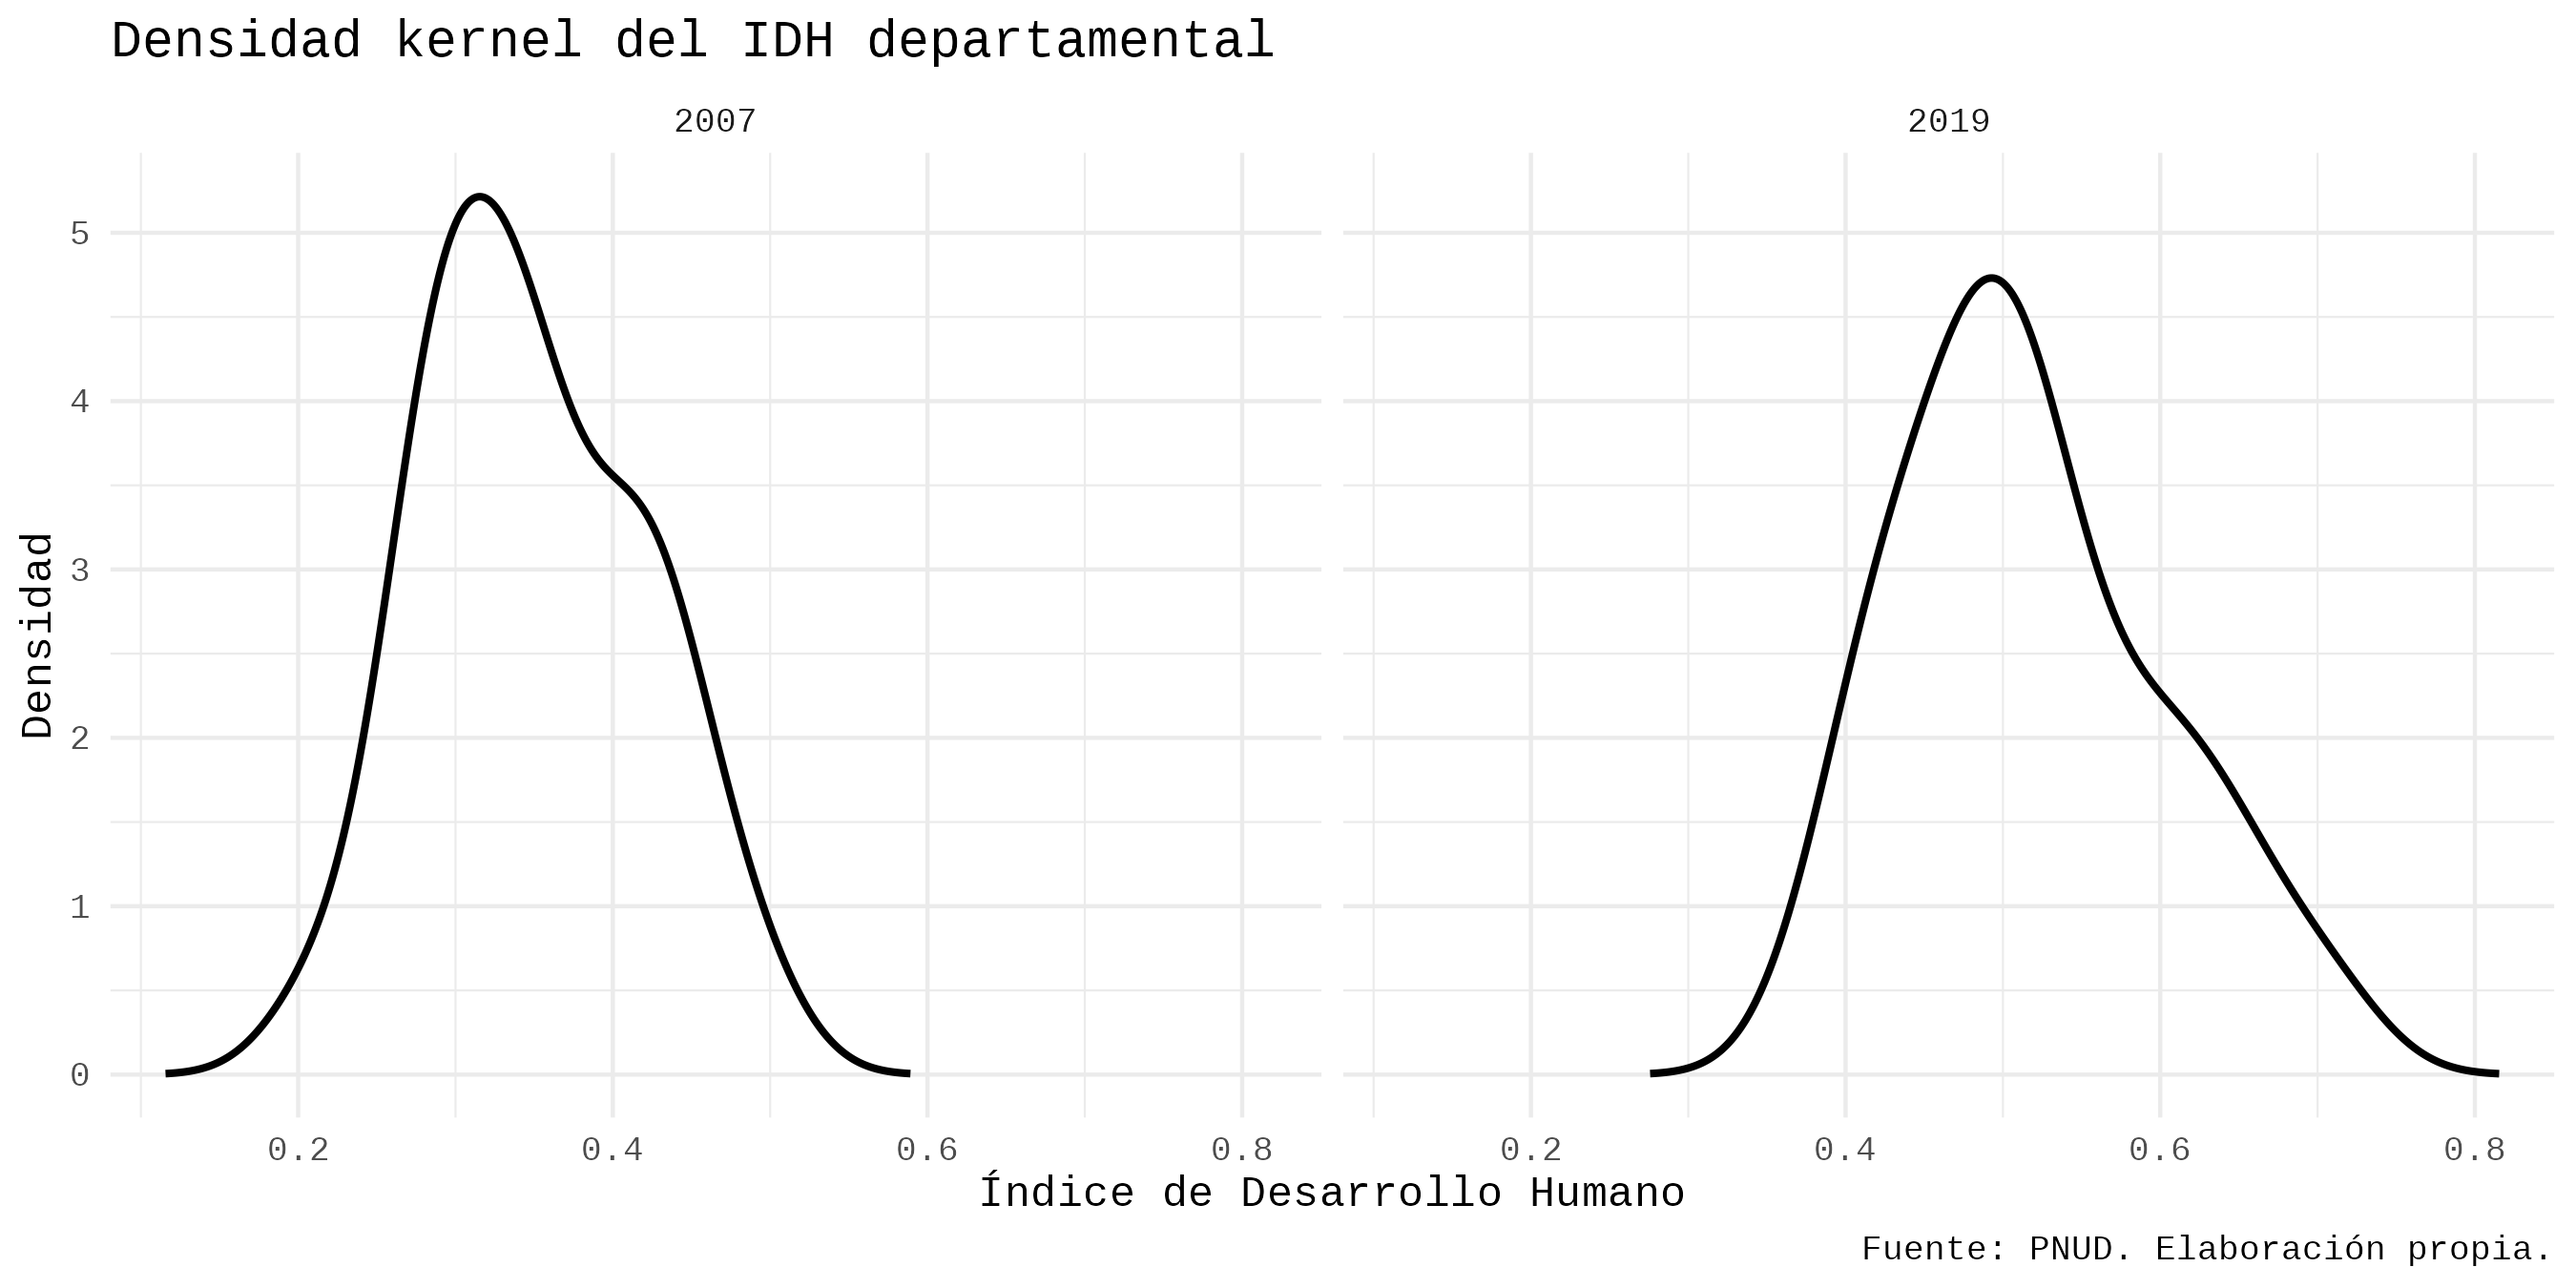
\includegraphics[width=0.88\textwidth]{figura_1_densidad_idh.png}
\caption{Distribución kernel del Índice de Desarrollo Humano, 2007 y 2019}
\label{fig:densidad_idh}
\begin{flushleft}
\footnotesize
\textit{Nota.} Las curvas representan densidades kernel departamentales.
El desplazamiento hacia la derecha indica una mejora general de los niveles
de desarrollo humano.
\end{flushleft}
\end{figure}

La Figura \ref{fig:mapas_idh} muestra la distribución territorial del IDH
inicial y de su cambio acumulado. Los niveles iniciales evidencian diferencias
persistentes entre los departamentos, mientras que el mapa de variaciones
permite observar que los avances no se distribuyeron de manera uniforme. La
existencia de mejoras generalizadas no elimina, por tanto, las diferencias en
la intensidad con la que cada territorio amplió sus capacidades.

\begin{figure}[H]
\centering
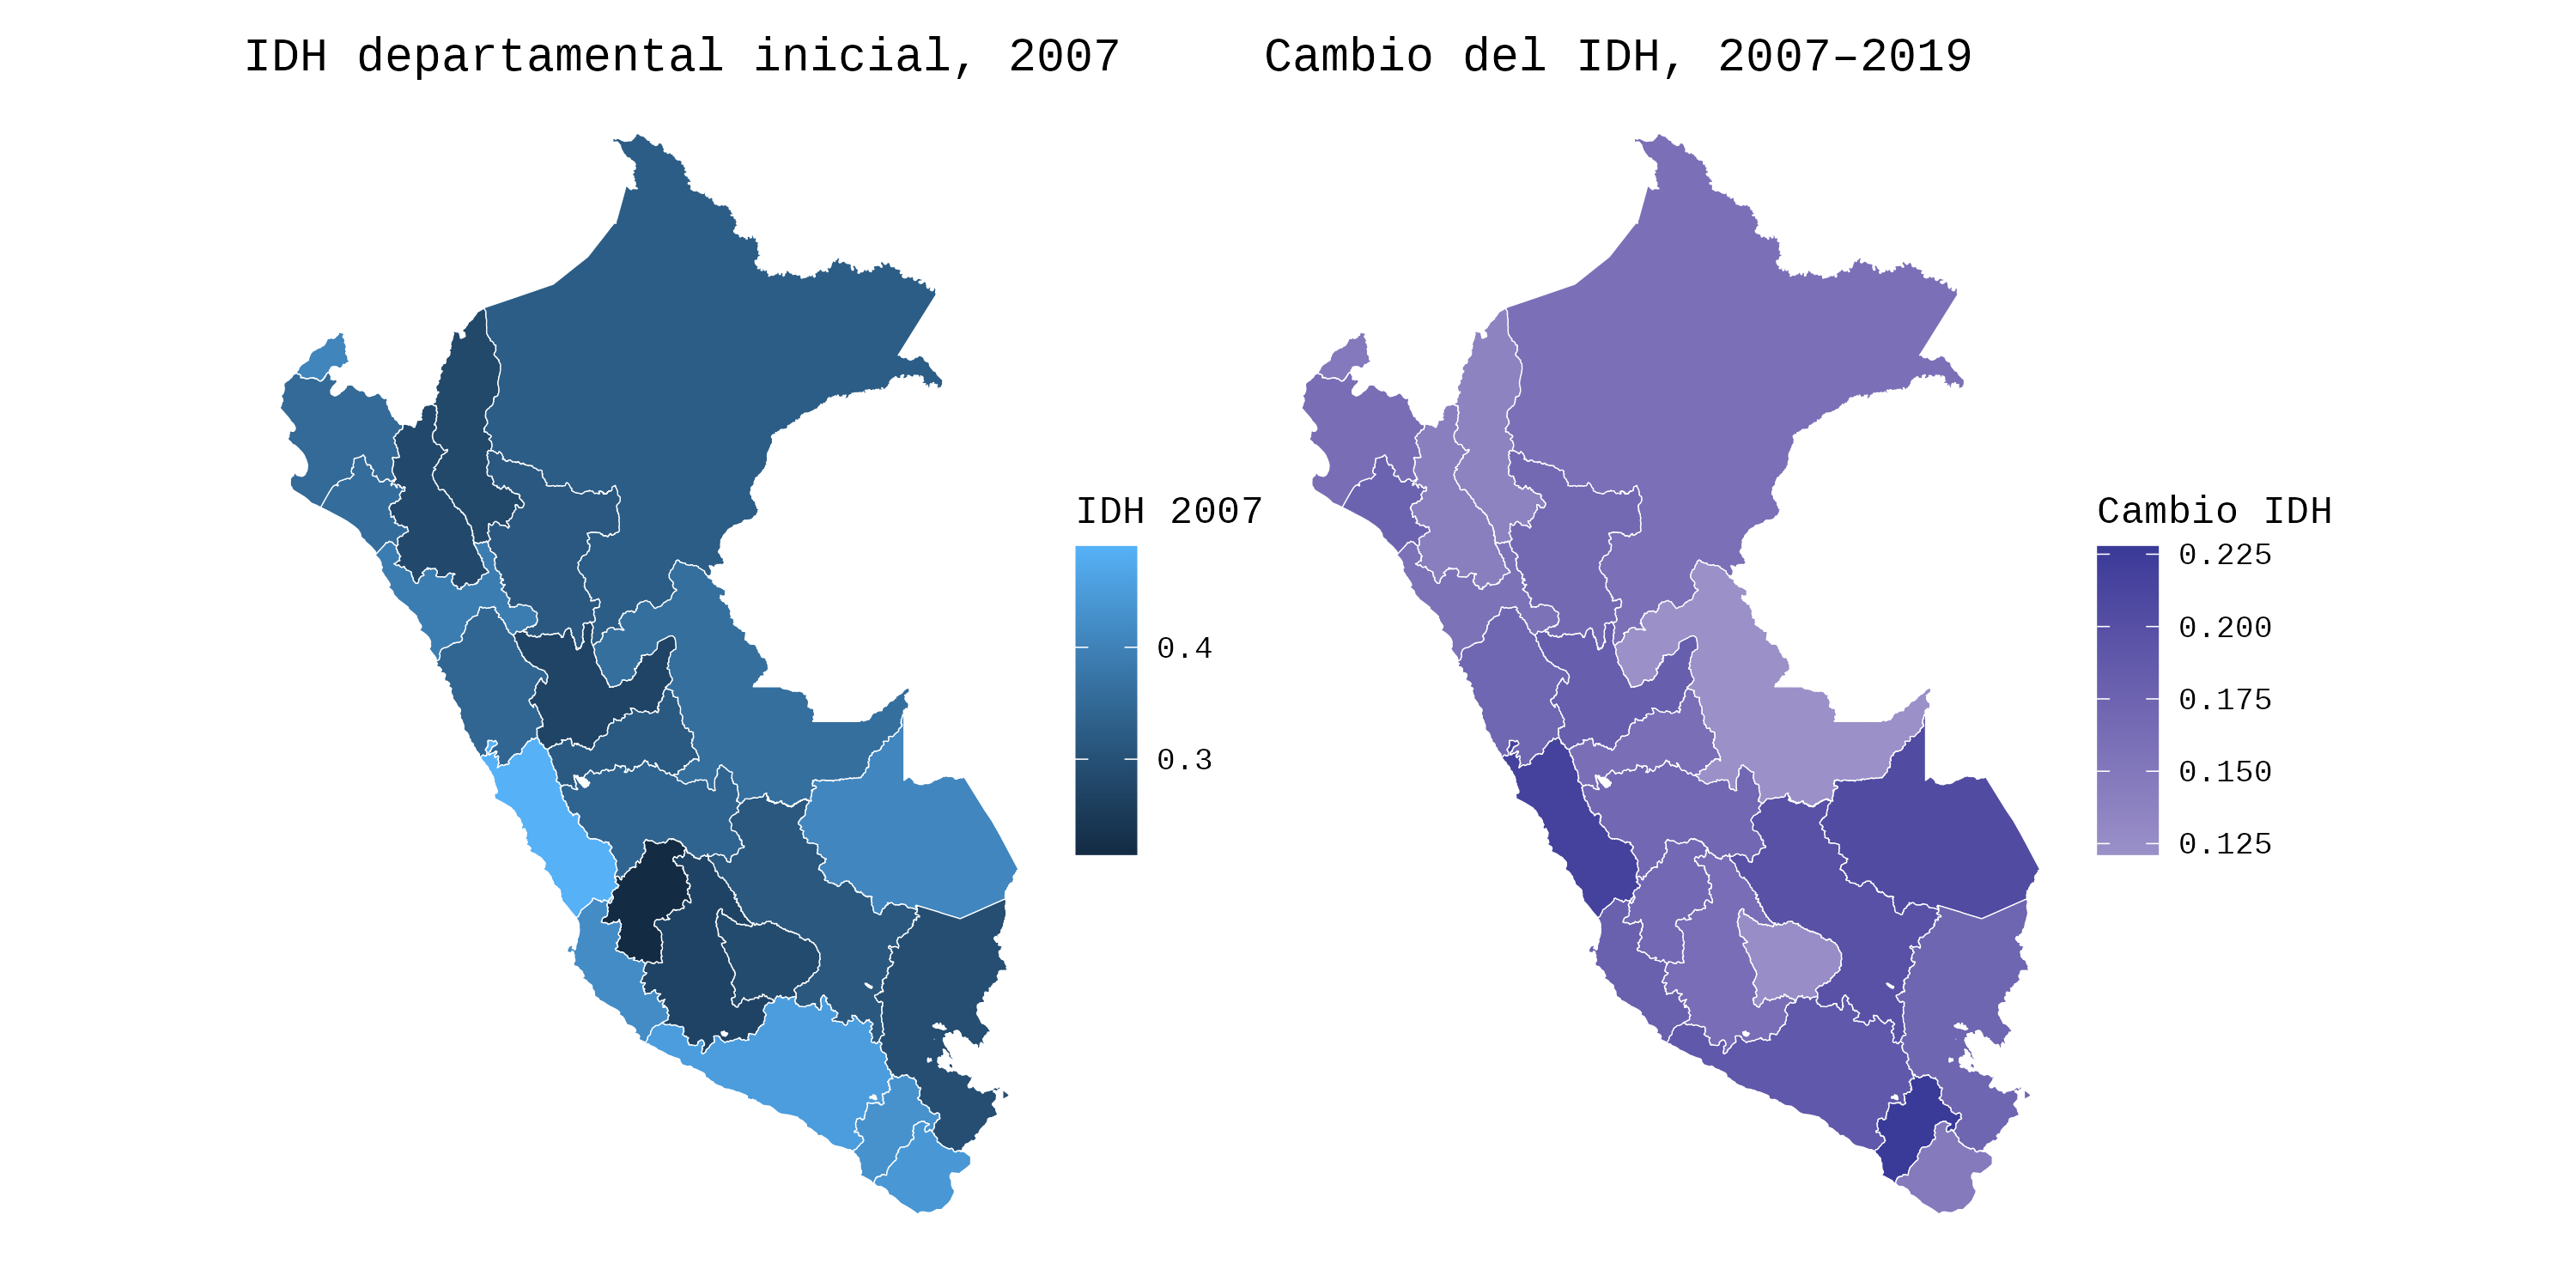
\includegraphics[width=0.94\textwidth]{figura_2_mapas_idh.png}
\caption{Distribución departamental del IDH inicial y su cambio acumulado}
\label{fig:mapas_idh}
\begin{flushleft}
\footnotesize
\textit{Nota.} El panel inicial representa los niveles departamentales de
2007; el segundo muestra la variación acumulada entre 2007 y 2019.
\end{flushleft}
\end{figure}

\subsection{Autocorrelación espacial global}

Los resultados del índice global de Moran se presentan en la Tabla
\ref{tab:moran_global}. Ninguno de los estadísticos estimados resulta
significativo al 5\%. Para la matriz de banda de distancia inversa, el Moran
del IDH inicial es $-0.0273$ y el correspondiente a su cambio acumulado es
$-0.0662$. En ambos casos, los valores de probabilidad son ampliamente
superiores a 0.05.

En el PBI per cápita relativo inicial, el Moran alcanza 0.0692, pero tampoco es
estadísticamente significativo. El cambio económico presenta un valor de
$-0.0769$, igualmente no significativo. Por tanto, no se identifica un patrón
global estable mediante el cual departamentos con valores similares se
encuentren sistemáticamente próximos entre sí.

Los resultados del IDH se mantienen cuando se utilizan las matrices de
contigüidad queen y cuatro vecinos más próximos. Esta estabilidad sugiere que
la ausencia de autocorrelación global no depende exclusivamente de la matriz
principal. No obstante, la inexistencia de asociación global significativa no
descarta la presencia de relaciones locales o de heterogeneidad en los
coeficientes regionales.

\begin{table}[H]
\centering
\caption{Índice global de Moran}
\label{tab:moran_global}
\small
\begin{tabular}{llrr}
\toprule
\textbf{Variable} &
\textbf{Matriz} &
\textbf{Moran $I$} &
\textbf{$p$-valor} \\
\midrule
IDH 2007               & Banda inversa & $-0.0273$ & 0.4443 \\
Cambio del IDH          & Banda inversa & $-0.0662$ & 0.5796 \\
$\ln$ PBIpc 2007        & Banda inversa & 0.0692    & 0.1581 \\
Cambio de $\ln$ PBIpc   & Banda inversa & $-0.0769$ & 0.6265 \\
IDH 2007                & Queen         & $-0.0690$ & 0.5752 \\
Cambio del IDH          & Queen         & $-0.0277$ & 0.4525 \\
IDH 2007                & KNN, $k=4$    & $-0.0713$ & 0.5903 \\
Cambio del IDH          & KNN, $k=4$    & $-0.0799$ & 0.6194 \\
\bottomrule
\end{tabular}
\begin{flushleft}
\footnotesize
\textit{Nota.} La hipótesis nula corresponde a ausencia de autocorrelación
espacial global. Ningún resultado es significativo al 5\%.
\end{flushleft}
\end{table}

El diagrama de dispersión espacial de la Figura \ref{fig:moran_idh} confirma
que los departamentos se distribuyen entre los distintos cuadrantes sin
formar un agrupamiento global claramente dominante. La pendiente de la recta
corresponde al índice de Moran y se mantiene próxima a cero.

\begin{figure}[H]
\centering
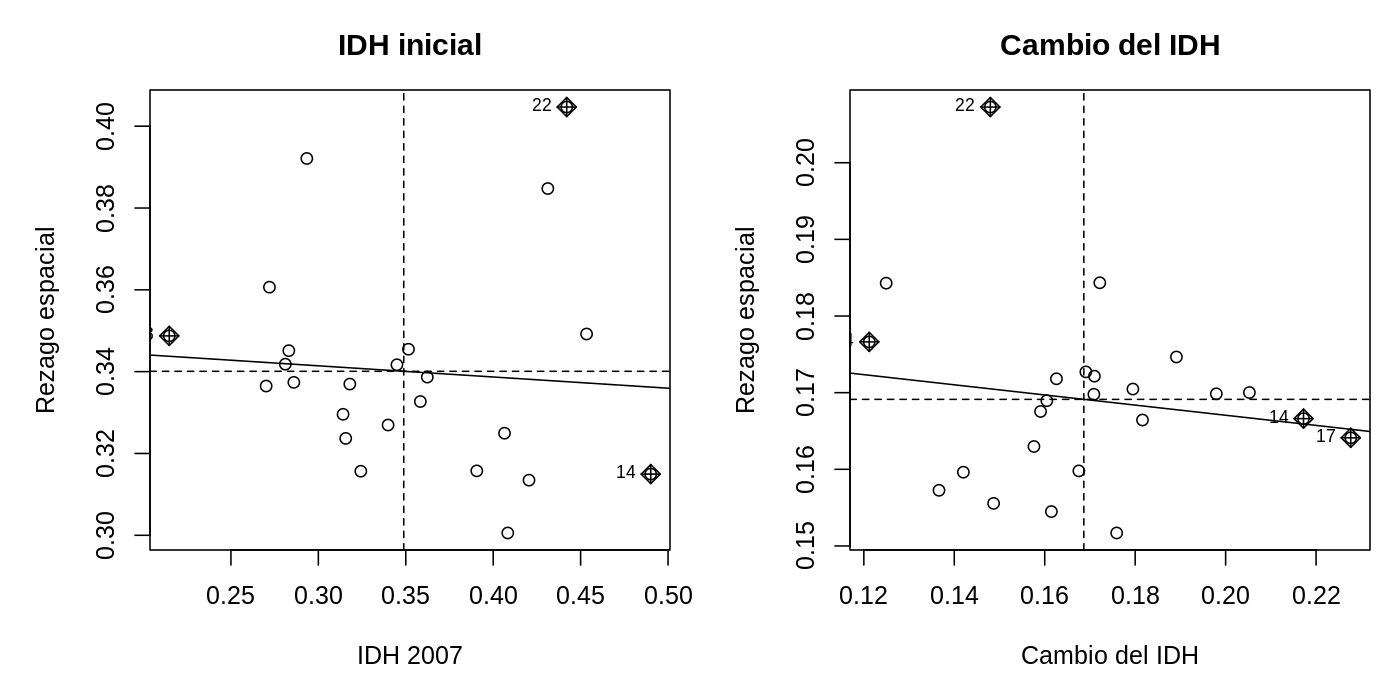
\includegraphics[width=0.90\textwidth]{figura_3_moran_scatter.png}
\caption{Diagramas de dispersión de Moran para el IDH}
\label{fig:moran_idh}
\begin{flushleft}
\footnotesize
\textit{Nota.} Los ejes representan el valor estandarizado del indicador y
su rezago espacial. La pendiente corresponde al índice global de Moran.
\end{flushleft}
\end{figure}

\subsection{Convergencia beta global}

Los resultados de las regresiones globales evidencian comportamientos
diferenciados entre desarrollo humano e ingreso regional. En la estimación
OLS del IDH, el coeficiente asociado con el nivel inicial es positivo y
estadísticamente significativo:

\begin{equation}
\widehat{\Delta IDH_i}
=
0.1115
+
0.1637 IDH_{i,2007}.
\end{equation}

El coeficiente de 0.1637 presenta un valor de probabilidad de 0.0355. Esto
significa que los departamentos con mayor IDH inicial registraron, en promedio,
incrementos superiores durante 2007--2019. Por consiguiente, no se encuentra
evidencia de convergencia beta del desarrollo humano. El resultado es más
compatible con una dinámica de divergencia beta o de persistencia acumulativa,
a pesar de que el coeficiente de variación disminuyó.

El modelo OLS del IDH alcanza un $R^2$ de 0.1858 y un $R^2$ ajustado de
0.1488. El nivel explicativo es moderado, lo que indica que una proporción
importante de las variaciones departamentales responde a factores no incluidos
en una regresión basada únicamente en el nivel inicial.

En contraste, el coeficiente del PBI real per cápita relativo inicial es
negativo y altamente significativo:

\begin{equation}
\widehat{\Delta x_i}
=
0.0229
-
0.3282 x_{i,2007}.
\end{equation}

El coeficiente de $-0.3282$ presenta un valor de probabilidad inferior a
0.001. Esto implica que los departamentos con una posición económica inicial
más rezagada mejoraron relativamente más que los departamentos inicialmente
adelantados. Por tanto, se identifica convergencia beta económica durante
2007--2019.

El modelo económico alcanza un $R^2$ de 0.4404 y un $R^2$ ajustado de 0.4150.
La velocidad anual implícita de convergencia, calculada a partir del coeficiente
OLS, es aproximadamente:

\begin{equation}
v
=
-\frac{\ln(1-0.3282)}{12}
=
0.0331.
\end{equation}

Por tanto, la velocidad estimada de convergencia económica es cercana al
3.3\% anual. Este resultado debe interpretarse como una aproximación promedio
para el conjunto departamental y no como una tasa uniforme para todos los
territorios.

\subsection{Modelos espaciales y robustez}

La Tabla \ref{tab:modelos_regresion} compara las estimaciones OLS, SEM y
Durbin-SEM. En el caso del IDH, el coeficiente inicial permanece positivo y
significativo bajo todas las especificaciones. Con la matriz de banda inversa,
el SEM estima un coeficiente de 0.1712, mientras que con la matriz queen el
valor asciende a 0.1882. Los resultados confirman que la ausencia de
convergencia beta del IDH no depende del modelo elegido.

El parámetro asociado con el rezago espacial del IDH inicial no es
significativo en la matriz de distancia. En la especificación queen alcanza
0.2782 y presenta un valor de probabilidad de 0.0710, por lo que solo sería
significativo bajo un criterio del 10\%. El AIC más bajo continúa
correspondiendo al OLS, aunque la diferencia respecto del Durbin-SEM queen es
reducida.

Para el PBI per cápita relativo, todos los modelos mantienen un coeficiente
inicial negativo y altamente significativo. En el SEM con banda inversa, el
coeficiente alcanza $-0.3666$, mientras que en el SEM queen asciende en valor
absoluto a $-0.3792$. El modelo queen presenta el menor AIC del conjunto
económico, con un valor de $-1.3505$.

Los coeficientes de los rezagos espaciales del nivel inicial no son
significativos al 5\%. En la matriz de distancia, el rezago del PBI inicial
alcanza un valor de 0.2323 con $p=0.0932$, mientras que en la matriz queen el
coeficiente es 0.1979 con $p=0.2704$. En consecuencia, la evidencia de
desbordamientos directos provenientes del nivel inicial de los departamentos
vecinos es limitada.

La comparación entre matrices muestra que la importancia de la dependencia
espacial es sensible a la definición de vecindad. La banda inversa no mejora el
AIC respecto del OLS, mientras que la contigüidad queen produce una mejora
considerable en el modelo económico. Por ello, la conclusión central se apoya
en la estabilidad del coeficiente de convergencia y no únicamente en la
selección de una especificación espacial particular.

\begin{table}[H]
\centering
\caption{Resultados de los modelos globales y espaciales}
\label{tab:modelos_regresion}
\scriptsize
\resizebox{\textwidth}{!}{
\begin{tabular}{llrrrrrr}
\toprule
\textbf{Variable} &
\textbf{Modelo} &
\textbf{$\beta$ inicial} &
\textbf{$p(\beta)$} &
\textbf{Rezago inicial} &
\textbf{$p$ rezago} &
\textbf{$\lambda$} &
\textbf{AIC} \\
\midrule
\multirow{5}{*}{Cambio IDH}
& OLS
& 0.1637 & 0.0355 & --- & --- & --- & $-106.4696$ \\

& SEM, banda inversa
& 0.1712 & 0.0123 & --- & --- & $-0.3166$ & $-105.2509$ \\

& Durbin-SEM, banda inversa
& 0.1698 & 0.0139 & 0.0317 & 0.8515 & $-0.3321$ & $-103.2841$ \\

& SEM, queen
& 0.1882 & 0.0063 & --- & --- & $-0.3117$ & $-105.3478$ \\

& Durbin-SEM, queen
& 0.1782 & 0.0064 & 0.2782 & 0.0710 & $-0.4470$ & $-106.2370$ \\
\midrule
\multirow{5}{*}{Cambio $\ln$ PBIpc}
& OLS
& $-0.3282$ & 0.0004 & --- & --- & --- & 2.3566 \\

& SEM, banda inversa
& $-0.3666$ & $<0.001$ & --- & --- & 0.3036 & 3.2253 \\

& Durbin-SEM, banda inversa
& $-0.3471$ & $<0.001$ & 0.2323 & 0.0932 & 0.1120 & 3.0383 \\

& SEM, queen
& $-0.3792$ & $<0.001$ & --- & --- & 0.6304 & $-1.3505$ \\

& Durbin-SEM, queen
& $-0.3439$ & $<0.001$ & 0.1979 & 0.2704 & 0.5564 & $-0.4129$ \\
\bottomrule
\end{tabular}
}
\begin{flushleft}
\footnotesize
\textit{Nota.} $\beta$ corresponde al coeficiente del nivel inicial.
El rezago inicial representa la variable explicativa espacialmente rezagada.
Los valores de $\lambda$ corresponden al parámetro del error espacial.
\end{flushleft}
\end{table}

\subsection{Heterogeneidad espacial de los coeficientes}

La regresión geográficamente ponderada permite evaluar si la relación entre el
nivel inicial y el cambio acumulado varía entre departamentos. Los diagnósticos
se presentan en la Tabla \ref{tab:diagnostico_gwr}.

Para el IDH, el ancho de banda seleccionado es de aproximadamente 1919.1 km,
equivalente a más del 100\% de la distancia máxima considerada en el
procedimiento. Asimismo, los coeficientes locales se encuentran entre 0.1625 y
0.1652, con un rango de apenas 0.0027. Estos resultados indican que la GWR del
IDH se comporta prácticamente como una regresión global. No se detecta una
heterogeneidad territorial relevante en la pendiente estimada.

En el PBI per cápita relativo, el ancho de banda disminuye a 360.5 km, lo que
representa aproximadamente 19.1\% de la distancia máxima. Los coeficientes
locales varían entre $-0.4857$ y $-0.2771$, con un rango de 0.2086. Todos los
coeficientes conservan signo negativo, pero la intensidad de la convergencia
cambia entre departamentos.

La existencia de coeficientes económicos negativos en todo el territorio
confirma que la convergencia no depende únicamente de un reducido grupo de
departamentos. Sin embargo, la magnitud más intensa en determinadas zonas
sugiere que las condiciones productivas, la accesibilidad, la estructura
económica y la articulación regional influyen en la velocidad con la que los
territorios modifican su posición relativa.

\begin{table}[H]
\centering
\caption{Diagnóstico de las regresiones geográficamente ponderadas}
\label{tab:diagnostico_gwr}
\small
\begin{tabular}{lrrrrr}
\toprule
\textbf{Variable} &
\textbf{Banda, km} &
\textbf{Proporción máxima} &
\textbf{$\beta$ global} &
\textbf{$\beta$ local mínimo} &
\textbf{$\beta$ local máximo} \\
\midrule
IDH
& 1919.1 & 1.0142 & 0.1637 & 0.1625 & 0.1652 \\

PBI per cápita
& 360.5 & 0.1905 & $-0.3282$ & $-0.4857$ & $-0.2771$ \\
\bottomrule
\end{tabular}
\begin{flushleft}
\footnotesize
\textit{Nota.} La proporción máxima relaciona el ancho de banda seleccionado
con la distancia máxima entre los centroides departamentales.
\end{flushleft}
\end{table}

La Figura \ref{fig:gwr_paneles} representa los coeficientes locales y los
niveles de ajuste de las estimaciones. En el IDH se observa una superficie
prácticamente uniforme, coherente con el reducido rango de las pendientes
locales. En el PBI per cápita aparecen diferencias territoriales más visibles,
aunque todos los coeficientes mantienen el signo compatible con convergencia.

\begin{figure}[H]
\centering
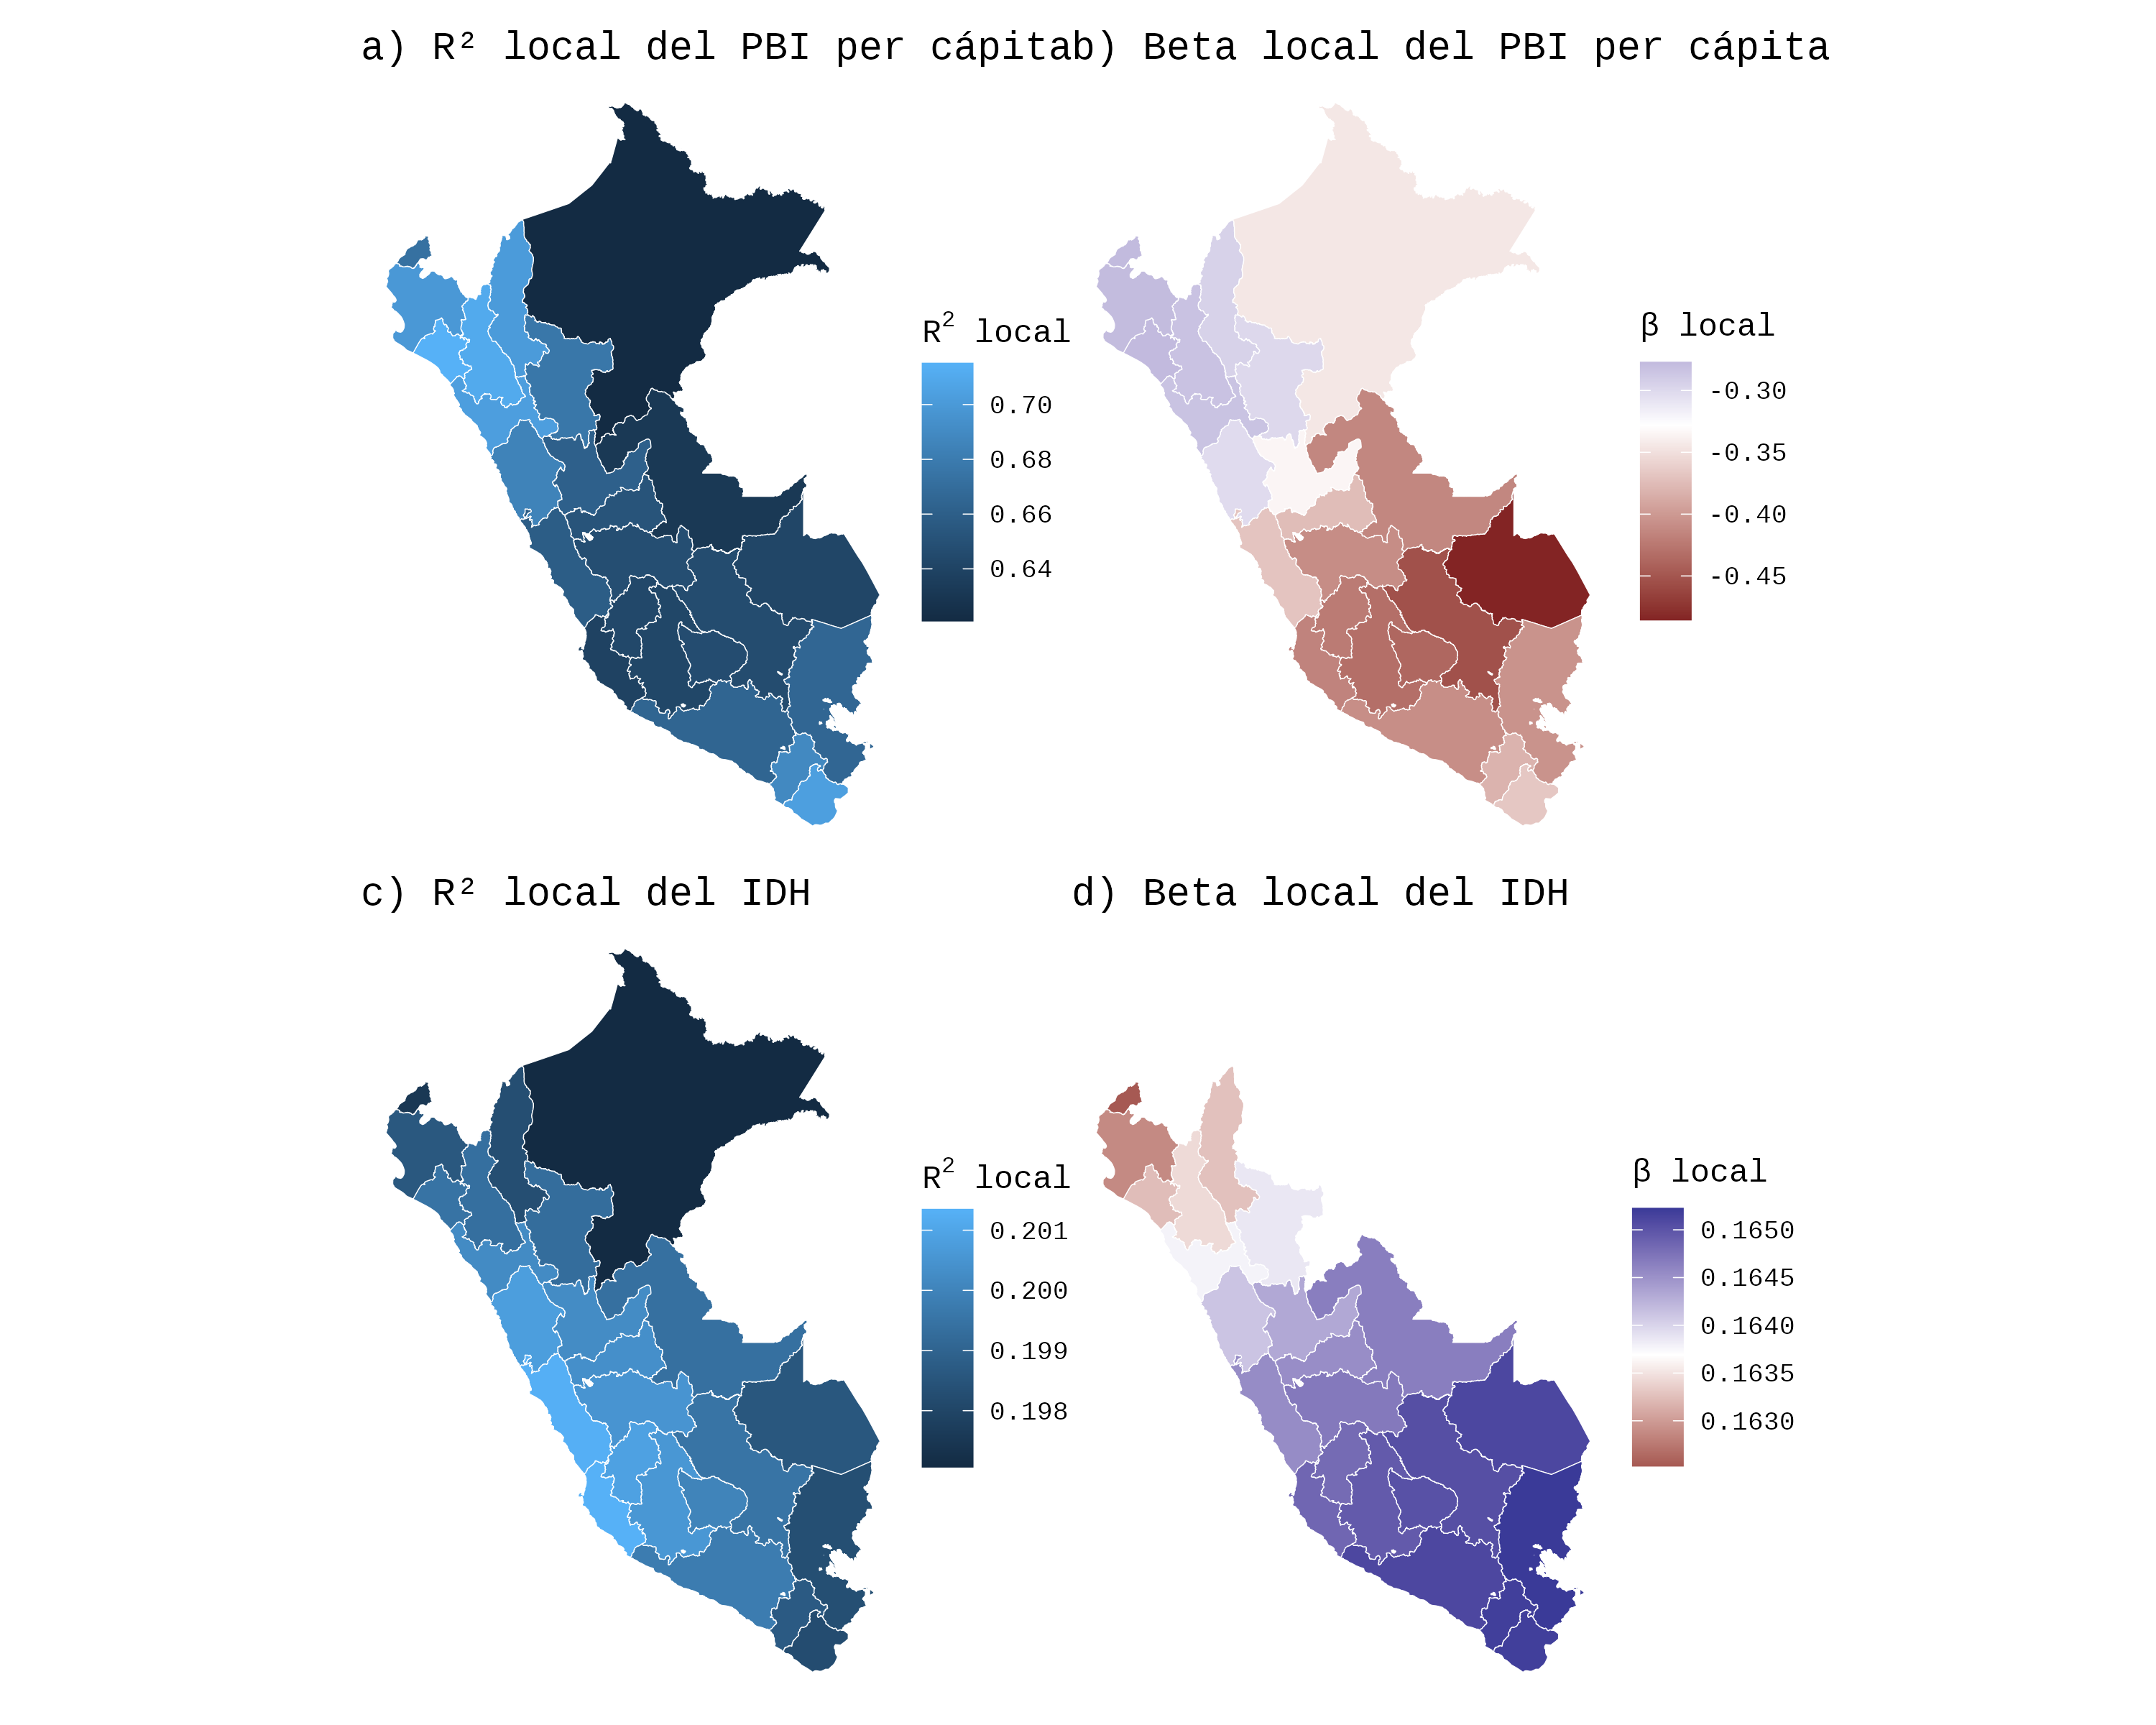
\includegraphics[width=0.96\textwidth]{figura_4_gwr_paneles.png}
\caption{Resultados territoriales de las regresiones geográficamente ponderadas}
\label{fig:gwr_paneles}
\begin{flushleft}
\footnotesize
\textit{Nota.} Los paneles muestran la distribución departamental del
coeficiente local y del ajuste de las regresiones GWR para el IDH y el PBI
real per cápita relativo.
\end{flushleft}
\end{figure}

Debido al reducido número de observaciones, estos resultados deben
interpretarse de manera exploratoria. Un ancho de banda amplio, como el
obtenido para el IDH, puede reflejar una relación verdaderamente global, pero
también puede estar asociado con una potencia estadística limitada para
detectar variaciones locales. Por esta razón, la escasa heterogeneidad
estimada no debe interpretarse como prueba definitiva de homogeneidad
territorial.

\subsection{Relaciones no paramétricas}

La Figura \ref{fig:no_parametricas} compara la regresión lineal con los
suavizamientos LOESS y kernel. En el IDH, las tres aproximaciones mantienen una
relación predominantemente positiva entre el nivel inicial y el cambio
acumulado. La coincidencia general de las curvas respalda la conclusión de
ausencia de convergencia beta.

En el PBI per cápita relativo, las estimaciones muestran una relación negativa.
Los departamentos con una posición inicial inferior presentan, en promedio,
una variación posterior mayor. Aunque las curvas no paramétricas revelan
cambios moderados en la pendiente, no alteran el signo central identificado por
los modelos globales.

La comparación entre ambos indicadores demuestra que la convergencia regional
no es un proceso uniforme entre dimensiones. La aproximación relativa del
ingreso departamental coexistió con una dinámica distinta en desarrollo
humano. Esto implica que los mecanismos que favorecen la reducción de las
brechas económicas no necesariamente producen resultados equivalentes en
educación, salud y capacidades humanas.

\begin{figure}[H]
\centering
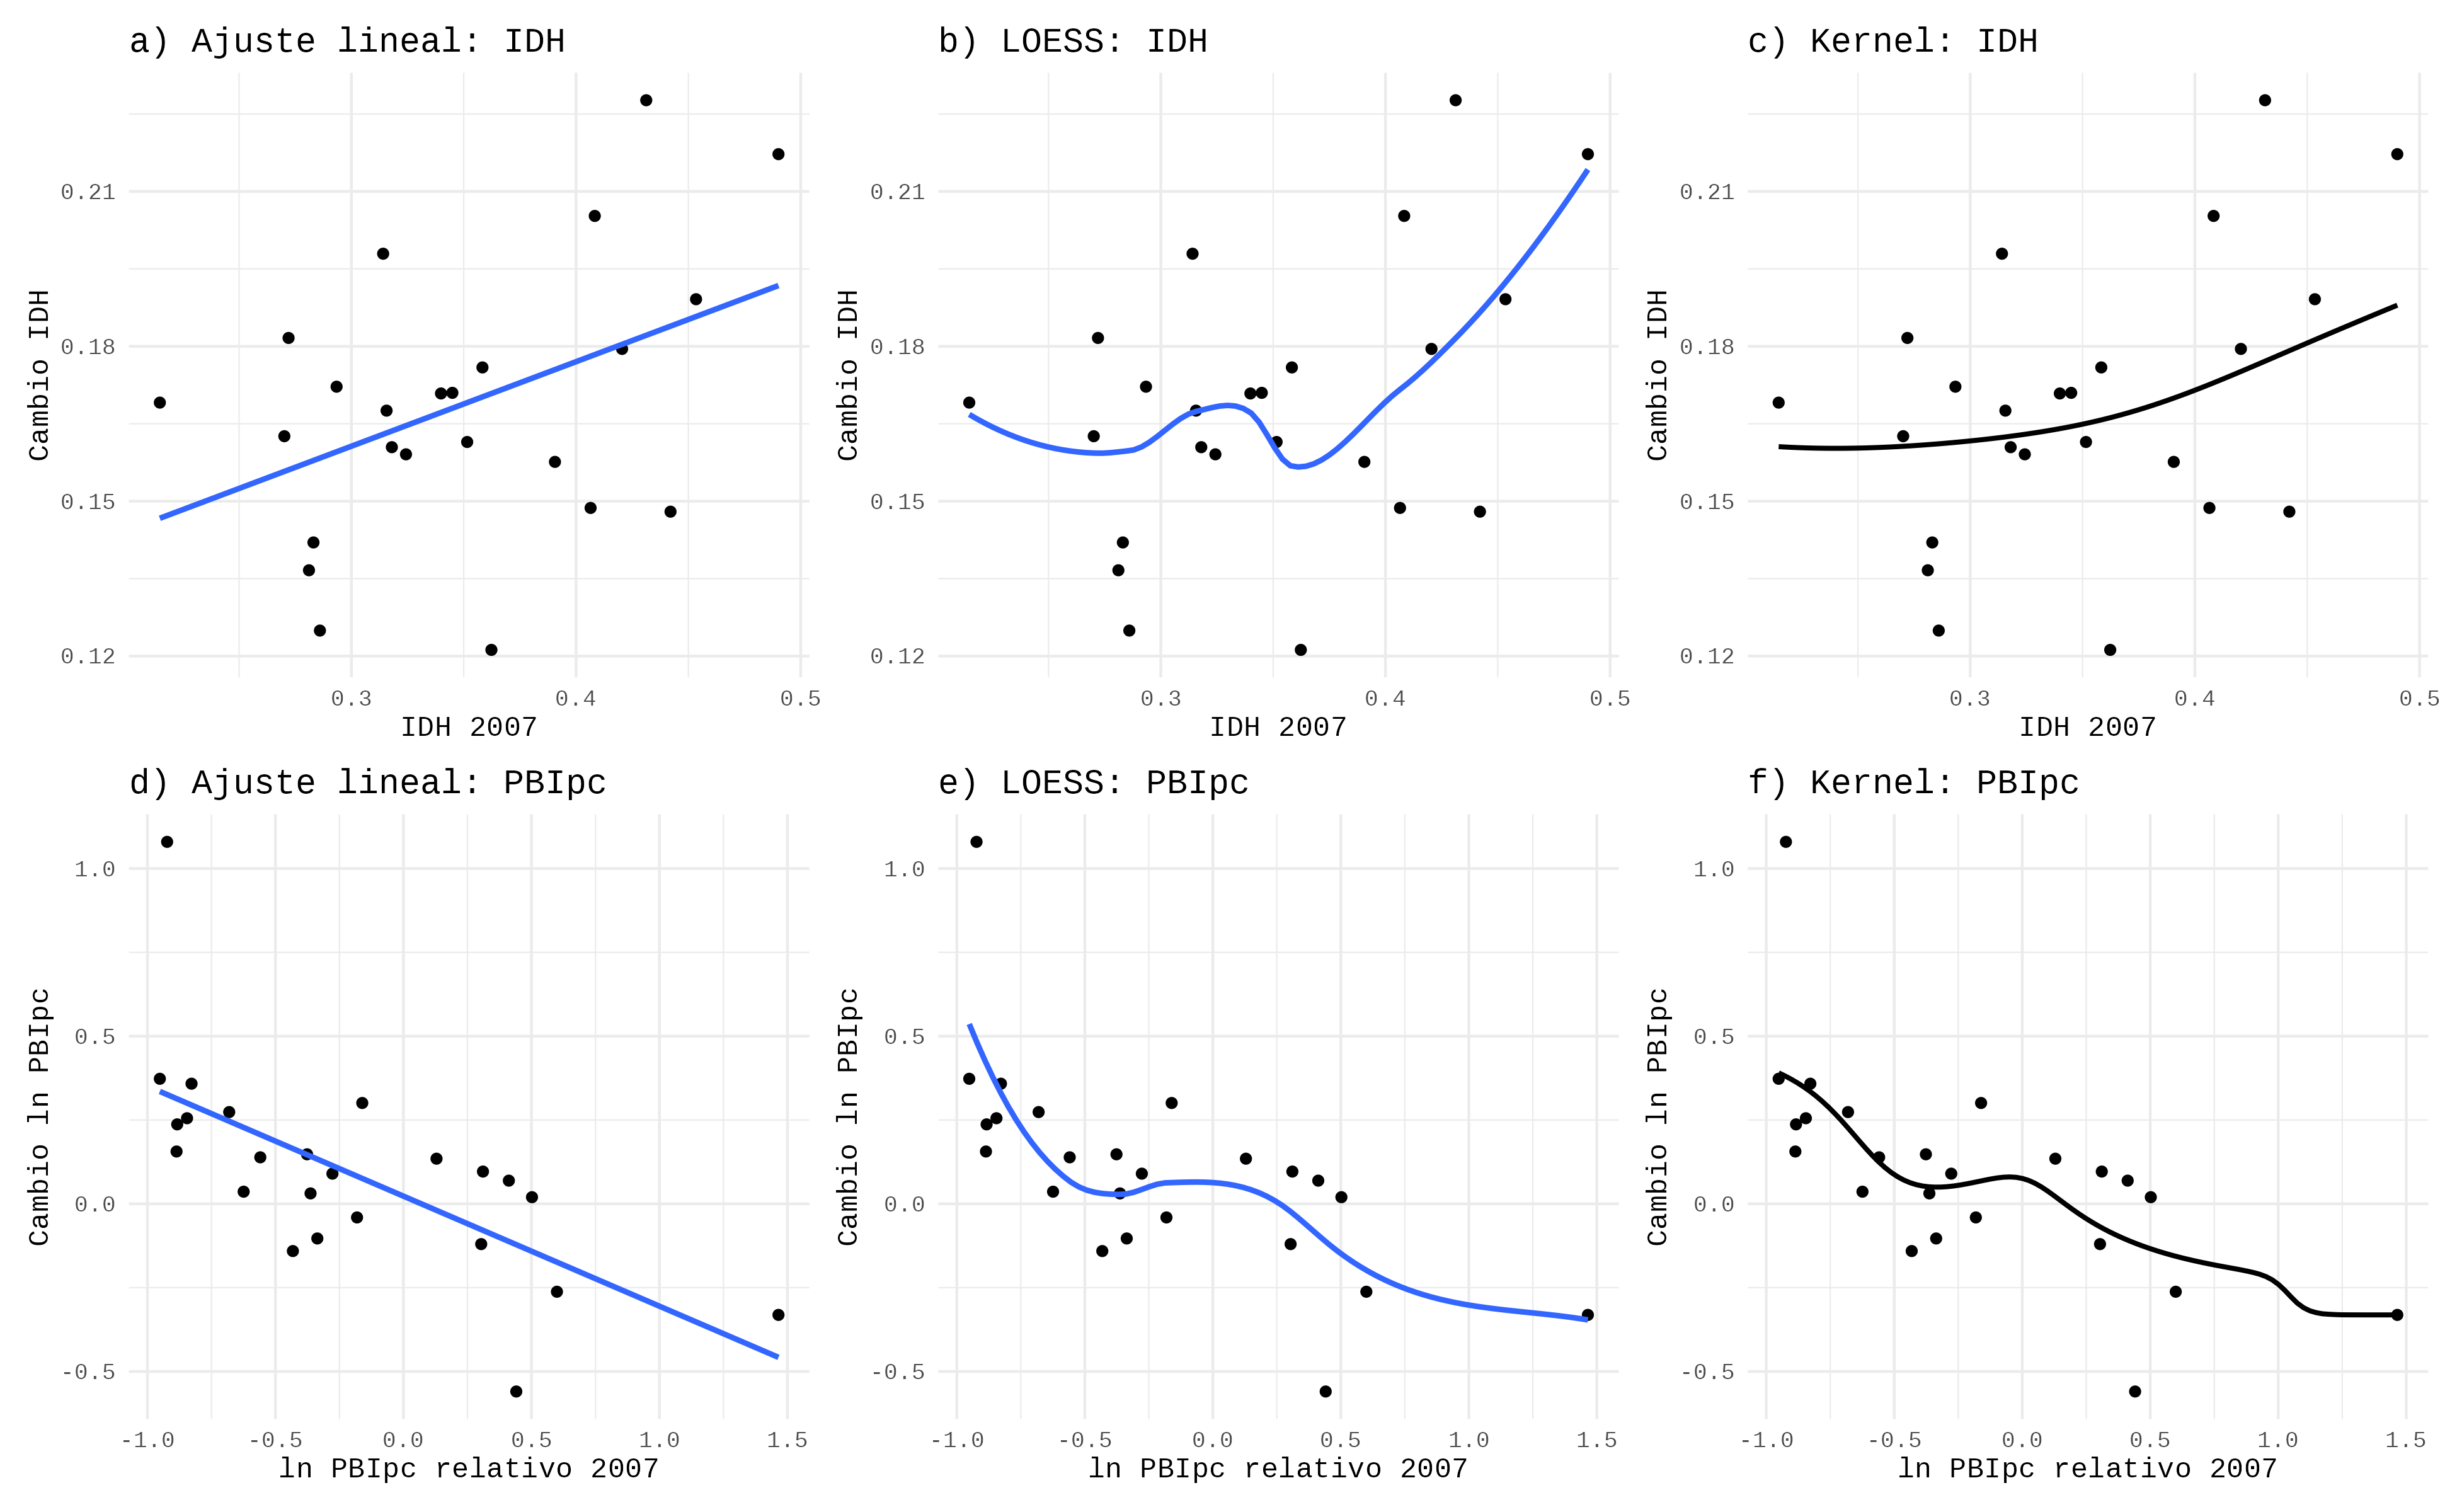
\includegraphics[width=0.96\textwidth]{figura_6_regresiones_no_parametricas.png}
\caption{Regresiones lineales y no paramétricas de convergencia}
\label{fig:no_parametricas}
\begin{flushleft}
\footnotesize
\textit{Nota.} Se comparan la recta OLS, el suavizamiento LOESS y la regresión
kernel para el IDH y el PBI real per cápita relativo.
\end{flushleft}
\end{figure}

\section{Discusión}

La dimensión que se utilice para medir las diferencias territoriales cambia
por completo la lectura de la convergencia regional en el Perú. El PBI real
per cápita relativo exhibe una relación negativa y estadísticamente
significativa entre el nivel inicial y el cambio acumulado; el IDH, en
cambio, exhibe el signo contrario. Durante 2007--2019, los departamentos se
acercaron entre sí en términos económicos sin que esa aproximación tuviera
una contraparte equivalente en desarrollo humano.
 
Ingreso y bienestar multidimensional rara vez avanzan al mismo compás. Un
territorio puede incrementar su producción por habitante sin que ese
crecimiento se traduzca de inmediato en mejores logros educativos, mejores
condiciones de salud o mayores oportunidades; esa traducción depende de la
provisión de servicios públicos, la infraestructura social, la calidad
institucional y la manera en que cada departamento distribuye internamente
sus recursos. El enfoque de capacidades sitúa precisamente ahí el punto
central: el crecimiento económico es un medio para ampliar las libertades de
la población, no una medida suficiente del desarrollo en sí misma
\parencite{sen1999}.
 
Que el coeficiente de variación del IDH haya disminuido podría interpretarse,
a primera vista, como una aproximación relativa entre departamentos. El signo
positivo del coeficiente beta obliga a matizar esa lectura: los territorios
que partían con niveles más altos también fueron los que más avanzaron. No
hay contradicción entre ambos resultados, porque responden a preguntas
distintas. La convergencia sigma describe cómo evoluciona la dispersión total
de la distribución; la convergencia beta pregunta si la posición inicial
predice el cambio posterior. Una distribución puede volverse menos dispersa
en términos relativos y, al mismo tiempo, conservar una ventaja dinámica para
quienes ya estaban mejor posicionados.
 
Esta distinción recupera un argumento planteado tempranamente por
\textcite{quah1993}: reducir la dinámica regional a un único coeficiente
puede ocultar más de lo que revela. Las densidades kernel, los mapas y las
regresiones no paramétricas de este estudio muestran precisamente eso: el
promedio nacional no resume el proceso departamental. El IDH mejoró en
términos agregados, pero las trayectorias individuales se mantuvieron
desiguales, con una relación positiva entre el punto de partida y el avance
posterior.
 
El coeficiente OLS de $-0.3282$ estimado para el PBI real per cápita
relativo, junto con la velocidad anual implícita de 3.3\%, constituye
evidencia de convergencia económica, aunque de un tipo particular: una
reducción de las posiciones relativas, no una igualación de niveles
absolutos. Los departamentos que partían rezagados mejoraron en promedio con
mayor rapidez que los que partían adelantados, sin que ello implicara el
cierre completo de las brechas productivas hacia el final del periodo.
 
La caída de la desviación estándar del indicador económico —de 0.6193 a
0.4750— respalda esta lectura y confirma una menor dispersión departamental.
Los valores extremos, sin embargo, siguen distantes entre sí, lo que revela
diferencias todavía relevantes en productividad, estructura sectorial y
capacidad de generación de ingresos. La convergencia observada es, en ese
sentido, un proceso parcial más que la desaparición de las desigualdades
regionales.
 
La literatura peruana sobre el tema anticipa buena parte de este patrón: las
conclusiones sobre convergencia dependen del periodo analizado, la variable
elegida y el método de estimación. \textcite{gonzales_trelles2004} ya habían
subrayado el peso de las diferencias territoriales y de la geografía
económica en la evolución regional; \textcite{palomino_rodriguez2019}
incorporaron la dependencia espacial al estudio del crecimiento
departamental; \textcite{pazparedes2023}, por su parte, identificó
trayectorias agrupadas y factores estructurales detrás de los clubes
regionales.
 
Ningún patrón espacial global resultó significativo para los niveles
iniciales ni para los cambios acumulados, lo que indica que los
departamentos con valores parecidos no se concentran de manera sistemática
en el territorio bajo las matrices empleadas. Eso no equivale a decir que el
espacio carezca de importancia: las pruebas LM, los modelos espaciales y la
GWR muestran que su relevancia cambia según el indicador y la definición de
vecindad que se utilice.
 
Para el IDH, los modelos espaciales conservan el signo positivo del
coeficiente inicial sin que los parámetros de error espacial ofrezcan
evidencia suficiente para desplazar al modelo OLS. El ancho de banda de la
GWR se aproxima además a la distancia máxima entre departamentos, y el rango
de los coeficientes locales es mínimo —señales que, en conjunto, apuntan a
una relación predominantemente global entre el nivel inicial del IDH y su
variación posterior.
 
Conviene, no obstante, ser cautelosos con esa lectura. Un ancho de banda tan
elevado puede reflejar una relación genuinamente homogénea en el territorio,
pero también puede ser síntoma de la limitada capacidad de una muestra de 24
departamentos para detectar variaciones locales. El resultado no demuestra,
entonces, que las dinámicas del desarrollo humano sean idénticas en todo el
país; solamente indica que la GWR empleada aquí no logra identificar
diferencias relevantes en la pendiente estimada.
 
La heterogeneidad espacial resulta bastante más visible en el PBI per
cápita relativo. Los coeficientes locales oscilan entre $-0.4857$ y
$-0.2771$ y conservan signo negativo en los 24 departamentos: hay
convergencia económica en todo el territorio, aunque su intensidad varía de
un lugar a otro. Este hallazgo coincide con lo planteado por
\textcite{duran2024}, para quienes los coeficientes globales pueden esconder
diferencias espaciales relevantes en la velocidad y la magnitud de la
convergencia.
 
También merece atención la sensibilidad de los modelos económicos frente a
la matriz espacial utilizada. La banda de distancia inversa no mejora el
criterio de información respecto del OLS, mientras que el SEM basado en
contigüidad queen sí presenta un AIC menor. Algunas pruebas robustas
detectan además dependencia en el componente de error, lo que sugiere que
las perturbaciones económicas comparten factores territoriales omitidos
entre departamentos vecinos —aunque la evidencia no es completamente
estable entre especificaciones.
 
Estas diferencias entre matrices no son un simple problema técnico. La
contigüidad captura vínculos fronterizos directos; la distancia inversa
asume que la interacción decae de forma continua conforme aumenta la
separación geográfica. En un territorio marcado por barreras naturales,
infraestructura desigual y conexiones económicas que no siempre coinciden
con la cercanía física, cada matriz termina representando un mecanismo de
interacción distinto.
 
En términos de política pública, una estrategia centrada únicamente en el
crecimiento económico regional difícilmente cerraría las brechas de
desarrollo humano. La convergencia del ingreso relativo necesita
complementarse con intervenciones en educación, salud, conectividad, empleo
de calidad y acceso a servicios básicos; la asignación de recursos debería
considerar tanto las condiciones iniciales de cada departamento como su
capacidad para transformar el crecimiento productivo en bienestar efectivo.
 
La heterogeneidad detectada en la convergencia económica pone en cuestión,
además, la aplicación uniforme de políticas regionales. Departamentos con
una convergencia más débil podrían requerir instrumentos específicos de
diversificación productiva, infraestructura logística y fortalecimiento del
capital humano, mientras que los vínculos entre territorios vecinos
justifican mecanismos de coordinación interdepartamental en transporte,
mercados, corredores productivos y provisión de servicios.
 
\subsection{Limitaciones del estudio}
 
El tamaño de la muestra es la limitación más evidente: 24 departamentos
restringen la potencia de las pruebas espaciales y de las regresiones
geográficamente ponderadas, por lo que los resultados locales deben leerse
como evidencia exploratoria y no como parámetros estructurales definitivos.
 
El nivel de agregación departamental plantea una segunda limitación, porque
puede esconder desigualdades internas entre provincias, distritos, zonas
urbanas y rurales. Dos departamentos con un promedio similar podrían
albergar distribuciones internas muy distintas; trabajos futuros con
información comparable podrían descender a unidades territoriales más
pequeñas.
 
Trabajar con dos momentos en el tiempo —2007 y 2019— permite estimar una
trayectoria acumulada, pero deja fuera las fluctuaciones intermedias. Un
panel anual habría permitido estimar efectos dinámicos, controlar
características no observadas y examinar cambios en la velocidad de
convergencia a lo largo del periodo.
 
También corresponde señalar una adaptación metodológica puntual: el IDH se
empleó directamente en su escala de cero a uno, en lugar de aplicar la
transformación utilizada en el estudio de referencia. La decisión facilita
la interpretación de los resultados, aunque limita la comparabilidad exacta
con otras réplicas del mismo ejercicio.
 
Por último, los modelos de convergencia incorporan únicamente el nivel
inicial como variable explicativa. Inversión pública, educación,
infraestructura, estructura productiva, urbanización, minería,
transferencias fiscales y calidad institucional podrían explicar una parte
adicional de las diferencias departamentales; su ausencia implica que los
resultados obtenidos identifican asociaciones de convergencia y no
relaciones causales.

\section{Conclusiones}

Esta investigación analizó las disparidades socioeconómicas y la
convergencia regional de 24 departamentos del Perú entre 2007 y 2019, a
partir del Índice de Desarrollo Humano y del PBI real per cápita relativo.
La estrategia combinó estadística descriptiva, densidades kernel,
cartografía, autocorrelación espacial, regresiones globales, modelos de
error espacial, especificaciones Durbin y regresiones geográficamente
ponderadas.
 
El resultado más llamativo del estudio es también el que le da su título de
trabajo: la aproximación económica entre departamentos no vino acompañada de
una convergencia equivalente en desarrollo humano. El IDH promedio subió de
0.3488 a 0.5175 y su coeficiente de variación cayó de 0.1986 a 0.1624 —una
reducción de la dispersión relativa compatible con convergencia sigma—, pero
la regresión beta arrojó un coeficiente positivo y significativo de 0.1637.
Los departamentos que partían con mejores condiciones fueron, en promedio,
los que más avanzaron; no hay evidencia, entonces, de convergencia beta en
desarrollo humano, aun cuando la brecha relativa se haya estrechado.
 
El PBI real per cápita relativo cuenta una historia distinta. Su desviación
estándar bajó de 0.6193 a 0.4750 y el coeficiente inicial de la regresión
OLS fue de $-0.3282$, significativo por debajo del 1\%, con una velocidad
anual implícita cercana a 3.3\%. Los departamentos que arrancaban rezagados
en términos económicos mejoraron su posición relativa con mayor rapidez que
los mejor posicionados, aunque las diferencias de nivel entre ellos
siguieran siendo importantes al cierre del periodo.
 
Ni los niveles iniciales ni los cambios acumulados mostraron autocorrelación
espacial global significativa: los índices de Moran se mantuvieron cercanos
a cero, con valores de probabilidad por encima del 5\%, y esa conclusión no
varió al cambiar la matriz de distancia inversa por contigüidad queen o por
cuatro vecinos próximos en el caso del IDH. La relevancia del espacio, sin
embargo, no desaparece por eso: reaparece con fuerza distinta según el
indicador que se examine. En el desarrollo humano, los modelos espaciales no
alteran el signo positivo del coeficiente y la GWR arroja pendientes locales
casi idénticas entre departamentos. En el PBI per cápita, en cambio, los 24
coeficientes locales son negativos pero varían entre $-0.4857$ y $-0.2771$
—hay convergencia económica en todo el territorio, aunque con una intensidad
que cambia de un lugar a otro.
 
La elección de la matriz de vecindad tampoco es un detalle menor: el modelo
de error con contigüidad queen ofrece un mejor ajuste para el PBI per
cápita que el basado en banda de distancia inversa, el cual ni siquiera
mejora al OLS según el criterio de Akaike. Esto sugiere que cualquier
lectura de la dependencia espacial en este tipo de ejercicios debería
apoyarse en más de una definición de proximidad geográfica antes de sacar
conclusiones firmes.
 
En conjunto, la evidencia describe una trayectoria dual —acercamiento
económico junto con persistencia de diferencias en desarrollo humano— que
tiene implicancias directas para el diseño de política. Reducir las brechas
de ingreso relativo no garantiza, por sí solo, una distribución más
equilibrada de las capacidades sociales; las políticas regionales necesitan
integrar crecimiento productivo con educación, salud, infraestructura,
empleo y acceso a servicios. La velocidad desigual de la convergencia
económica, además, exige que las estrategias de desarrollo se adapten a la
estructura productiva, la conectividad y las condiciones iniciales de cada
departamento, sin perder de vista que los vínculos entre territorios
vecinos justifican una coordinación interdepartamental en infraestructura,
corredores económicos, mercados laborales y provisión de servicios.
 
Quedan varias líneas abiertas para investigaciones posteriores: paneles
anuales que capturen la dinámica dentro del periodo, unidades territoriales
más desagregadas, variables estructurales adicionales, y una exploración
específica de clubes de convergencia y dependencia espacial local más allá
de 2019. Avanzar en esa dirección ayudaría a precisar por qué el
acercamiento económico departamental no se traduce, todavía, en una
convergencia equivalente del desarrollo humano.


\printbibliography[
  heading=bibintoc,
  title={Referencias}
]

\appendix
\section{Anexos}

\subsection{Distribución espacial del PBI real per cápita relativo}

\begin{figure}[H]
\centering
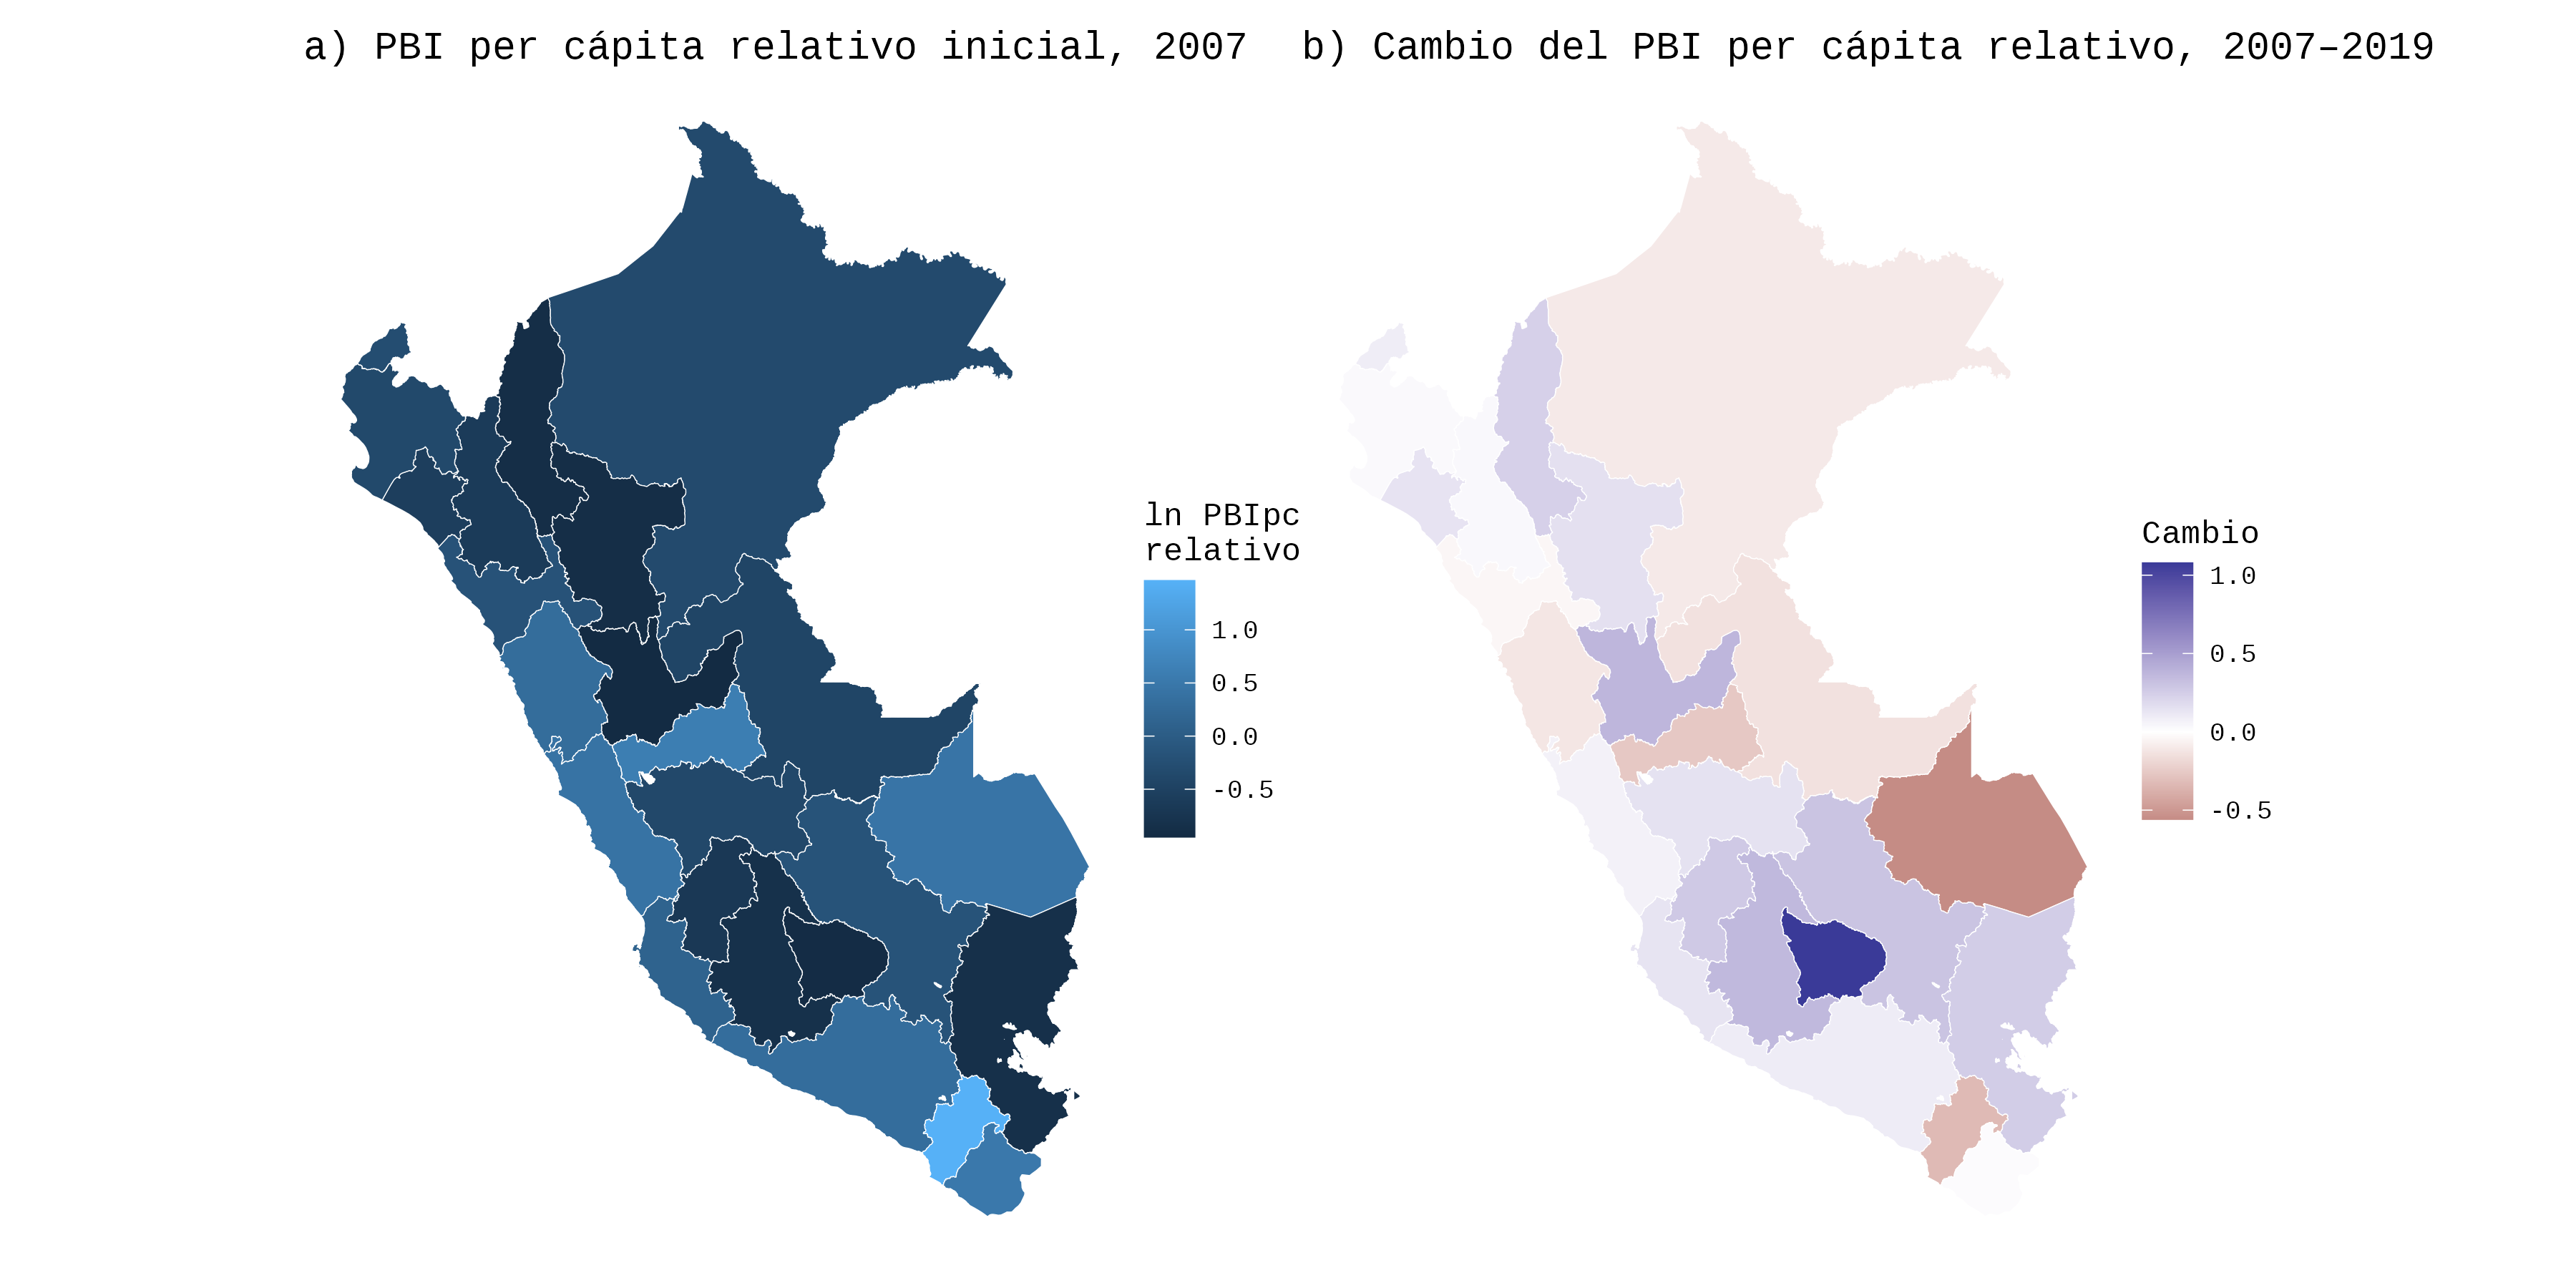
\includegraphics[width=0.94\textwidth]{figura_A1_mapas_pbi.png}
\caption{PBI real per cápita relativo inicial y cambio acumulado}
\label{fig:anexo_mapas_pbi}
\begin{flushleft}
\footnotesize
\textit{Nota.} El primer panel representa el logaritmo del PBI real per cápita
relativo en 2007 y el segundo su cambio acumulado entre 2007 y 2019.
\end{flushleft}
\end{figure}

\subsection{Dispersión espacial del PBI per cápita}

\begin{figure}[H]
\centering
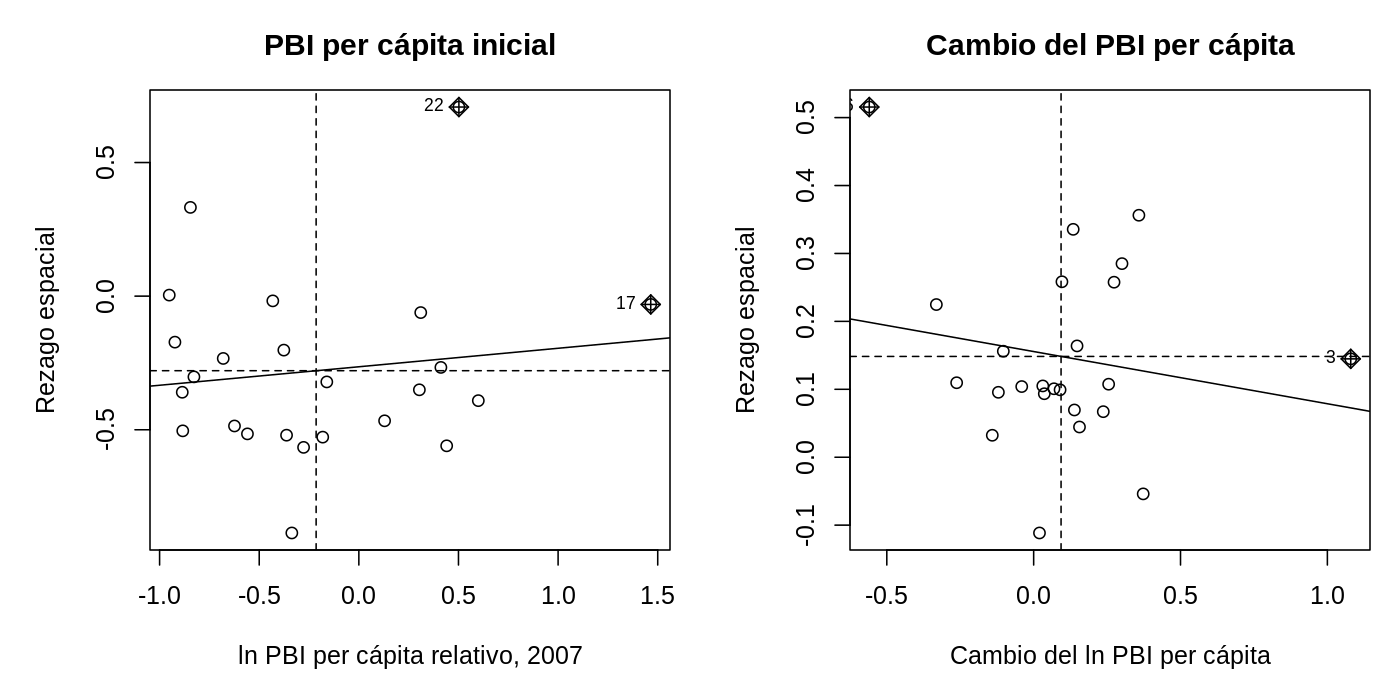
\includegraphics[width=0.90\textwidth]{figura_A2_moran_pbi.png}
\caption{Diagramas de dispersión de Moran para el PBI per cápita relativo}
\label{fig:anexo_moran_pbi}
\begin{flushleft}
\footnotesize
\textit{Nota.} Los diagramas corresponden al nivel inicial y al cambio
acumulado del indicador económico.
\end{flushleft}
\end{figure}

\subsection{Coeficientes locales de convergencia económica}

\begin{figure}[H]
\centering
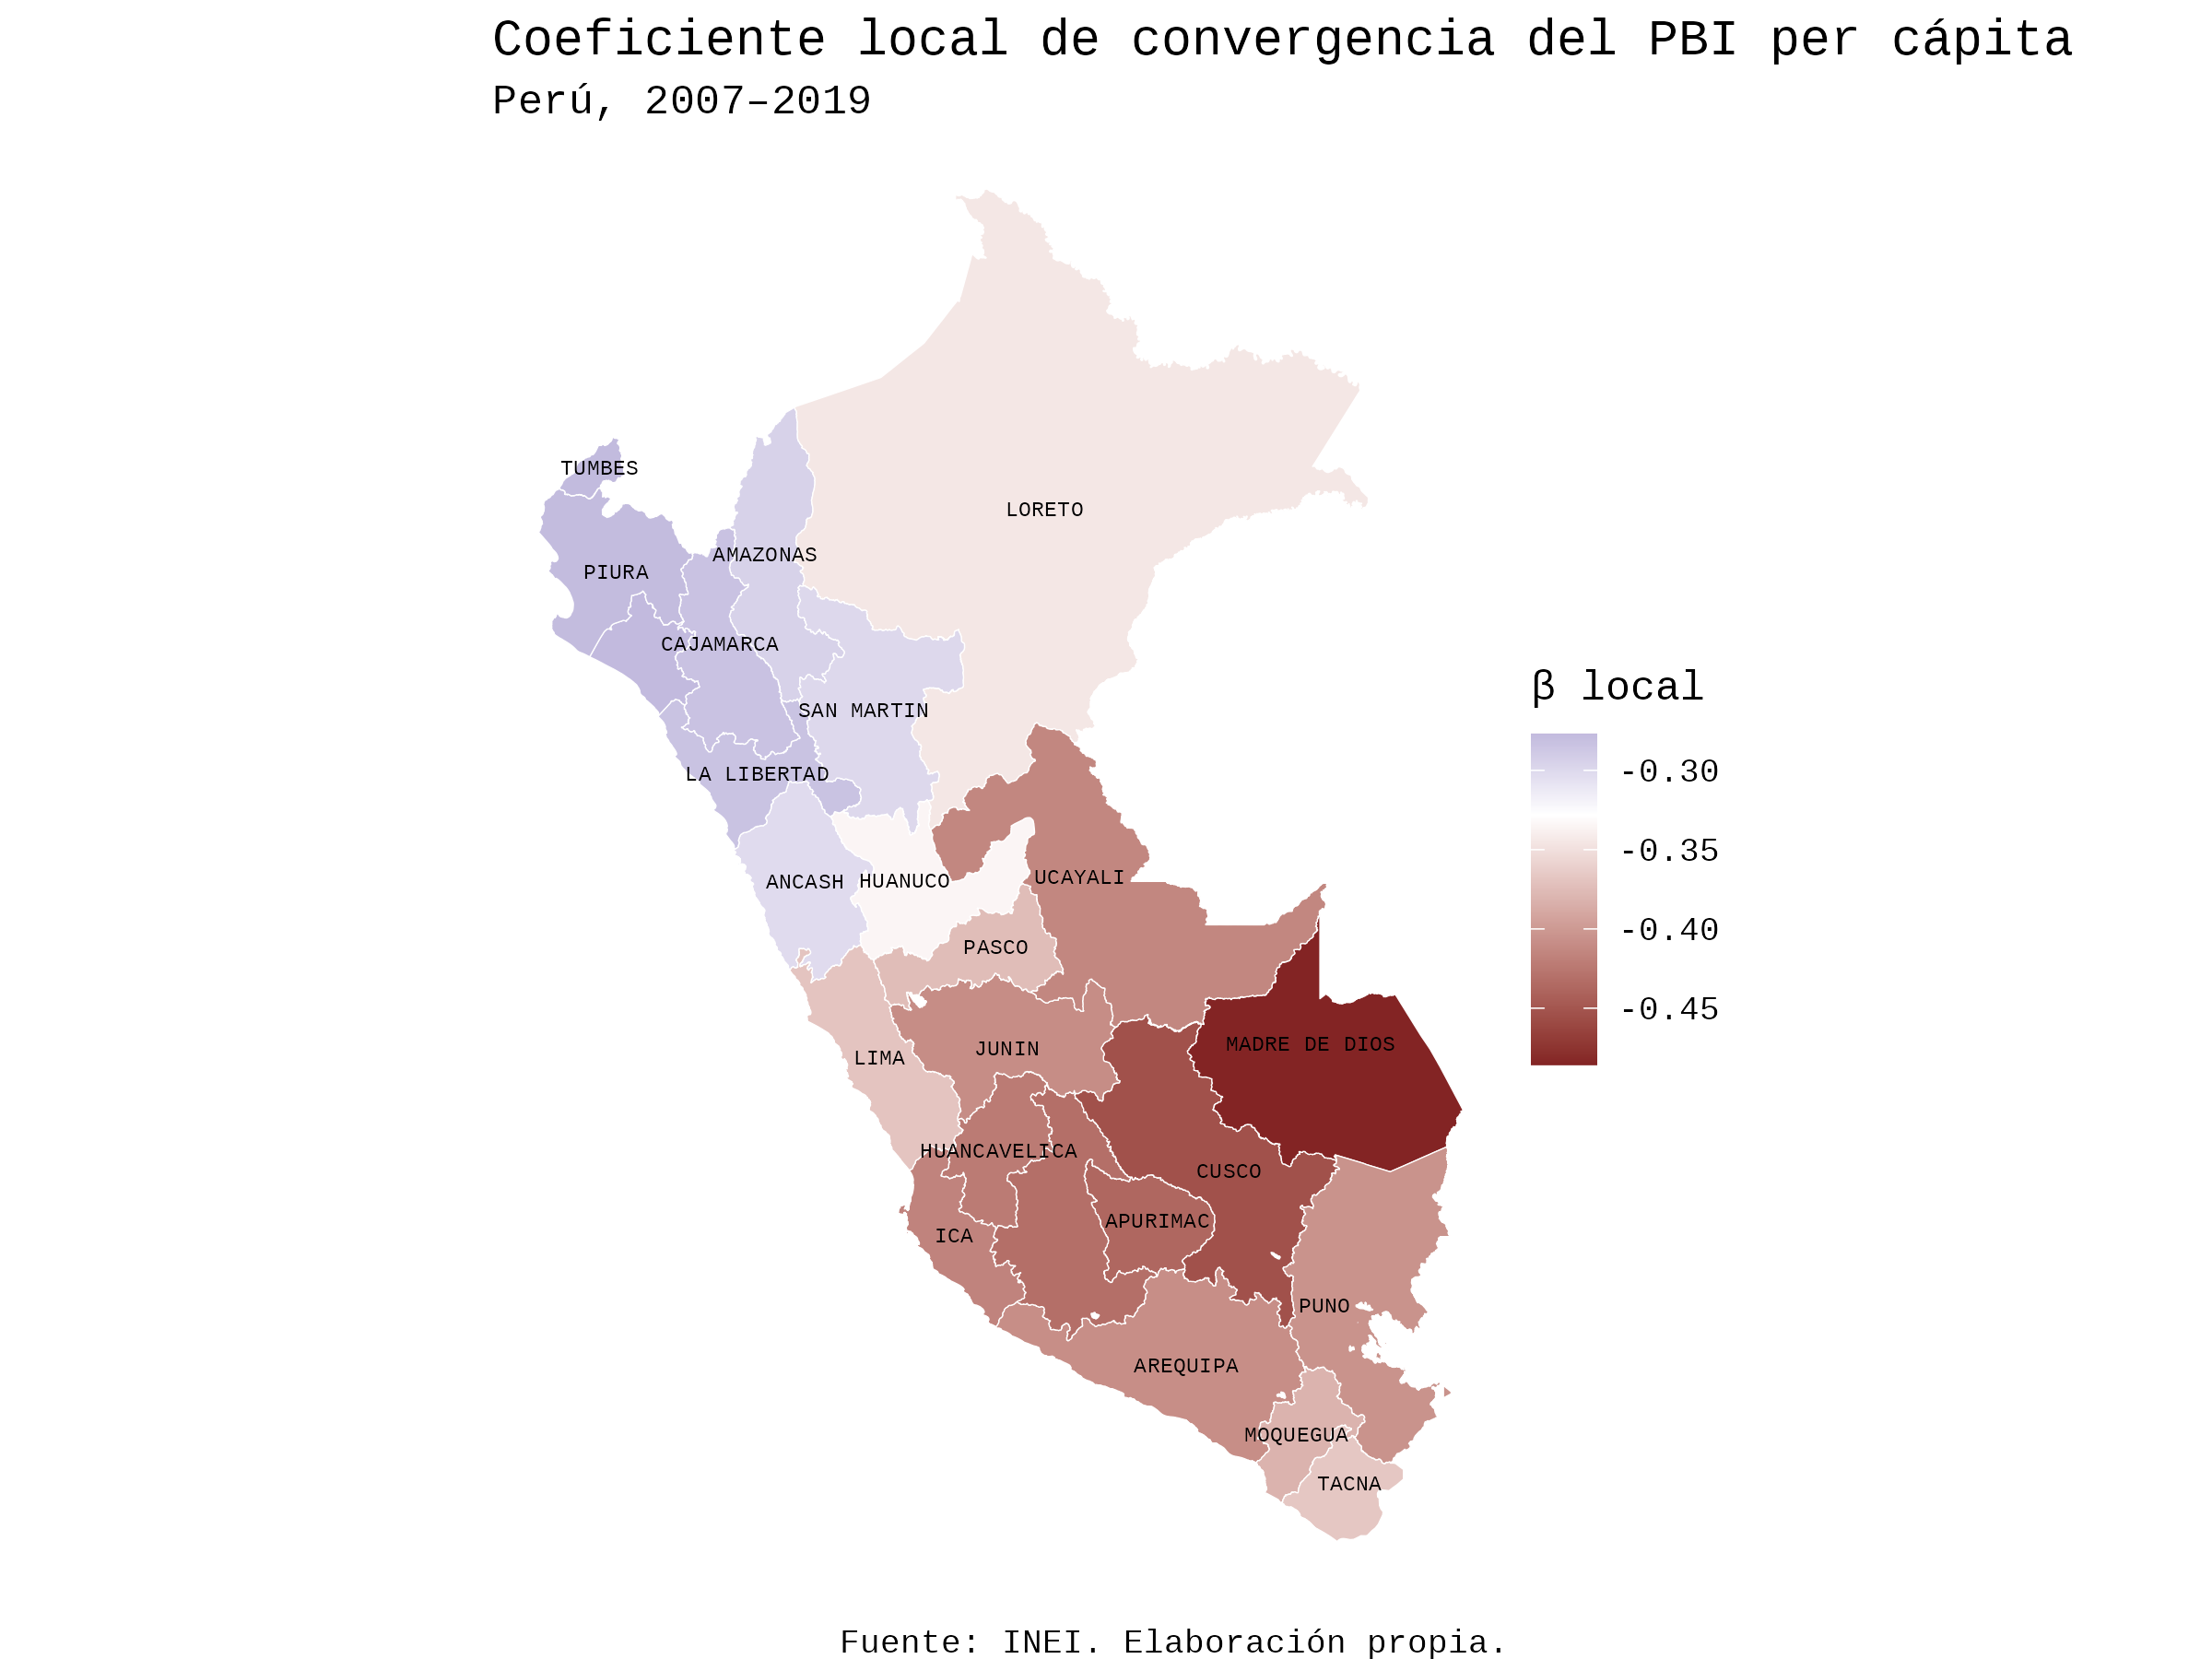
\includegraphics[width=0.78\textwidth]{figura_5_gwr_beta_pbi.png}
\caption{Distribución territorial del coeficiente local del PBI per cápita}
\label{fig:anexo_beta_pbi}
\begin{flushleft}
\footnotesize
\textit{Nota.} Los valores negativos representan convergencia beta. Una mayor
magnitud absoluta indica una convergencia local más intensa.
\end{flushleft}
\end{figure}

\subsection{Pruebas de dependencia espacial}

\begin{table}[H]
\centering
\caption{Pruebas LM/RS de dependencia espacial}
\label{tab:anexo_lm}
\scriptsize
\begin{tabular}{lllrr}
\toprule
\textbf{Variable} &
\textbf{Matriz} &
\textbf{Prueba} &
\textbf{Estadístico} &
\textbf{$p$-valor} \\
\midrule
Cambio IDH & Banda inversa & RS error ajustado & 0.0329 & 0.8560 \\
Cambio IDH & Banda inversa & RS rezago ajustado & 0.0008 & 0.9770 \\
Cambio IDH & Queen & RS error ajustado & 2.3093 & 0.1286 \\
Cambio IDH & Queen & RS rezago ajustado & 1.8635 & 0.1722 \\
\midrule
Cambio $\ln$ PBIpc & Banda inversa & RS error ajustado & 4.1951 & 0.0405 \\
Cambio $\ln$ PBIpc & Banda inversa & RS rezago ajustado & 2.9907 & 0.0837 \\
Cambio $\ln$ PBIpc & Queen & RS error ajustado & 6.2672 & 0.0123 \\
Cambio $\ln$ PBIpc & Queen & RS rezago ajustado & 2.9723 & 0.0847 \\
\bottomrule
\end{tabular}
\begin{flushleft}
\footnotesize
\textit{Nota.} Las pruebas robustas permiten distinguir entre dependencia
espacial en el error y dependencia asociada con el rezago espacial. Para el
PBI per cápita, la evidencia se concentra principalmente en el componente de
error.
\end{flushleft}
\end{table}


\end{document}
